% !TEX root = ../CA_book.tex

\chapter{테일러 급수와 로랑 급수}

이 장에서는 영역 $D$에 정의된 복소해석함수 $f$는 
$D$의 임의의 점에서 급수 전개가 가능하다는 근본적인 성질을 먼저 공부할 것이다.
다음 그림에서 왼쪽을 참고하라.
\begin{figure*}[h!]
\begin{center}
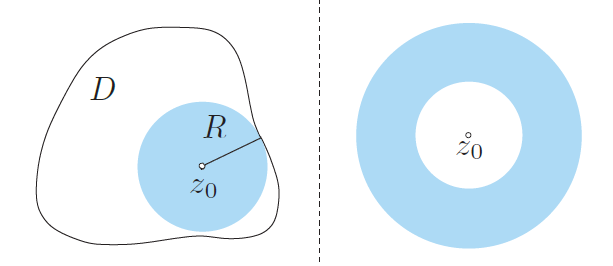
\includegraphics[width=0.5\textwidth]{./SaltChapter/fig-4-0-1}
\end{center}
\end{figure*}
\[
\text{테일러 급수: } \sum_{n=0}^\infty c_n(z-z_0)^n 
\quad
\text{로랑 급수: } \sum_{n\in \mathbb Z} c_n(z-z_0)^n 
\]

즉, 각각의 $z_0 \in D$에 대하여 다음을 만족하는 $R>0$이 존재한다.
\[
f(z) = \sum_{n=0}^\infty c_n(z-z_0)^n, \quad |z-z_0| <R.
\]
역으로,  적당한 $R$에 대하여 $|z-z_0|<R$을 만족하는 두 개 이상의 점에서 급수
\[
\sum_{n=0}^\infty c_n(z-z_0)^n
\]
가 수렴하면 $|z-z_0|<R$에서 복소해석함수이다.
이를 보이는 과정에서 복소해석함수에 대한 근본적인 성질들을 증명할 것이다.
\begin{itemize}
\item[(1)] (일반화된) 코시 적분공식과 코시 부등식
\item[(2)] 해의 분류와 항등정리
\item[(3)] 최대절대값정리
\end{itemize}

이 장의 후반부에서는
급수와 유사하지만 $z-z_0$ 항의 지수를 음의 정수까지 확장한
로랑 급수를 공부할 것이다.
이는 원환(특히 뚫린 원판)에 정의된 복소해석함수를 연구하는데 특히 유용하다,
앞의 그림에서 오른쪽을 참고하라.
끝으로 로랑 급수는 ``특이점''의 분류와 실함수 적분의 계산에도 유용함을 살펴볼 것이다.

\section{급수}

실수열의 경우와 유사하게 주어진
복소수열 $(a_n)_{n\in\mathbb N}$에 대하여
부분합 수열 $(s_n)_{n\in\mathbb N}$을 만들 수 있다.
\begin{align*}
s_1 &:= a_1, \\
s_2 &:= a_1 + a_2, \\
s_3 &:= a_1 + a_2 + a_3, \\
& \vdots
\end{align*}

\begin{saltdefinition} {}{} \label{def-4-1}

\begin{itemize}
\item[(1)] 복소수열 $(s_n)_{n\in\mathbb N}$이 수렴하면
$\sum\limits_{n=1}^\infty a_n := \lim\limits_{n\to\infty} s_n$라 쓰고
급수 $\sum\limits_{n=1}^\infty a_n$이 {\bf 수렴한다}고 정의한다.
\item[(2)] 복소수열 $(s_n)_{n\in\mathbb N}$이 발산하면,
급수 $\sum\limits_{n=1}^\infty a_n$는 {\bf 발산한다}고 정의한다.
\item[(3)] 실급수 $\sum\limits_{n=1}^\infty |a_n|$이 수렴하면,
급수 $\sum\limits_{n=1}^\infty a_n$은 {\bf 절대수렴한다}고 정의한다.
\end{itemize}
\end{saltdefinition}

복소수열이 수렴할 필요충분조건은
실수부와 허수부로 만든 수열이 각각 수렴하는 것이라는 
연습문제 \ref{ex-1-25}의 결과로부터,
\[
\sum\limits_{n=1}^\infty a_n\,\text{이 수렴한다. }
\Longleftrightarrow \text{\textcolor{red}{ 실수열} }
\sum\limits_{n=1}^\infty \Re(a_n)\, \text{과 }
\sum\limits_{n=1}^\infty \Im(a_n)\,\text{가 수렴한다.}
\]
따라서  실해석학의 결과를 아용하여 복소수열의 수렴성을 판정할 수 있다.
예를 들면, 다음 결과들을 쉽게 얻을 수 있는데 이는 연습문제로 남긴다.

\begin{salt_exercise}\label{ex-4-1}
$\Sum_{n=1}^\infty a_n$이 수렴하면, $\Lim_{n\to\infty}a_n = 0$임을 보여라.
\end{salt_exercise}

\begin{salt_exercise}\label{ex-4-2}
$\Sum_{n=1}^\infty a_n$이 절대수렴하면, $\Sum_{n=1}^\infty a_n$이 수렴함을 증명하라.
\end{salt_exercise}

\begin{salt_exercise}\label{ex-4-3}
$|z|<1$이면 $\Sum_{n=0}^\infty z^n$이 수렴하고 
$\Sum_{n=0}^\infty z^n = \dfrac1{1-z}$임을 보여라.
\end{salt_exercise}

\begin{salt_exercise}\label{ex-4-4}
$|z|<1$이면 $\Sum_{n=0}^\infty nz^{n-1} = \dfrac1{(1-z)^2}$임을 보여라.
\end{salt_exercise}

\begin{salt_exercise}\label{ex-4-5}
$\Re(s)>0$인 모든 복소수 $s\in \mathbb C$에 대하여
$1^{-s} +  2^{-s} + 3^{-s} + \cdots$가 수렴함을 보여라.
그러면
\[
s \mapsto \zeta(s) := \sum_{n=1}^\infty \dfrac1{n^s}
\]
\end{salt_exercise}
는 반평면 $\Re(s)>1$에서 잘 정의된 함수가 되며, 이를 
{\bf 리만 제타함수}라고 한다.
리만 제타함수와 정수론의 소수이론을 연결한 {\bf 오일러 곱셈공식}에 따르면,
소수를 증가하는 순서대로 나열한
$p_1:=2 < p_2:=3 < p_3:=5 < \cdots$를 무한 소수열로 정의할 때 다음이 성립한다.
\[
\zeta(s) = \lim_{K\to \infty} \prod_{k=1}^K \dfrac1{1-p_k^{-s}},
\quad \Re(s)>1.
\]
버나드 리만(1826-1866)은 제타함수 $\zeta$를 확장하여 $\mathbb C\setminus \{1\}$의 
복소해석함수로 정의할 수 있음을 보였다. 
$\zeta$는 $-2, -4, -6, \ldots$에서 ``자명해(trivial zero)''를 갖지면
다른 해도 존재한다. 리만이 계산한 모든 비자명해(nontrivial zero)는 모두 직선 $\Re(s) = 1/2$위에
있다. 이로부터 리만은 다음과 같이 예측(conjecture)하였는데 이는 여전히 수학계의 유명한 미해결 문제이다.

\begin{salt_conjecture}[리만가설] \label{conj-4-1}
리만 제타함수의 모든 비자명해는 직선 $\Re(s) = 1/2$ 위에 있다.
\end{salt_conjecture}

\section{급수}

\subsection{제곱급수와 수렴영역}

$(c_n)_{n\in\mathbb N}$을 복소수열이라고 하자.
다음과 같은 표현을
\[
\sum_{n=0}^\infty c_nz^n
\]
복소수 변수 $z$의 제곱급수라고 한다 ($(c_n)_{n\in\mathbb N}$을 계수들의 수열로 생각해도 된다).
이제 특정한 값을 급수의  $z$에 대입하는 경우를 생각해볼 수 있다.
그러면 어떤 $z\in\mathbb C$에 대하여 제곱급수가 수렴할 수 있고, 
다른 값에서는 발산할 수도 있다.

\begin{saltexample}[label=example-4-1]{}{}
모든 다항식은 유한개의 항에서만 계수가 $0$이 아닌 제곱급수 꼴로 쓸 수 있다.
따라서 다항식은 모든 $z\in\mathbb C$에 대하여 수렴한다.

제곱급수  
\[
\sum_{n=0}^\infty z^n
\]
는 $|z|<1$에서 수렴한다. 
$|z|\ge1$에서 급수는 발산한다 (왜냐하면 $\Lim_{n\to\infty} z^n = 0$이 성립하지 않으므로).
\hfill$\diamondsuit$
\end{saltexample}

근본적인 질문으로 
\begin{center}
어떤 $z\in\mathbb C$에 대하여  급수 $\sum_{n=0}^\infty c_nz^n$가 수렴하는가?
\end{center}

이 문제에 대한 답은 다음 정리에서 얻을 수 있다.

\begin{salttheorem}{}{} \label{thm-4-1}
제곱급수 $\Sum_{n=0}^\infty c_nz^n$에 대하여
다음 두 가지 중 정확히 하나만 성립한다.
\begin{itemize}
\item[(1)] 모든 $z\in\mathbb C$에 대하여 절대수렴하거나
\item[(2)] 음이 아닌 실수 $R$이 유일하게 존재하여 다음을 만족한다.
\begin{itemize}
\item[(a)] $|z|<R$인 모든 $z\in\mathbb C$에 대하여 $\Sum_{n=0}^\infty c_nz^n$이 절대수렴하고,
\item[(b)] $|z|>R$인 모든 $z\in\mathbb C$에 대하여 $\Sum_{n=0}^\infty c_nz^n$는 발산한다.
\end{itemize}
\end{itemize}
\end{salttheorem}

위 정리에서 유일한 $R>0$을 급수의 수렴반경이라 부른다.
급수가 모든 $z\in\mathbb C$에 대하여 수렴하면
무한대의 수렴반경을 가지며 ``$R=\infty$''라 쓴다.

\begin{figure}[h!]
\begin{center}
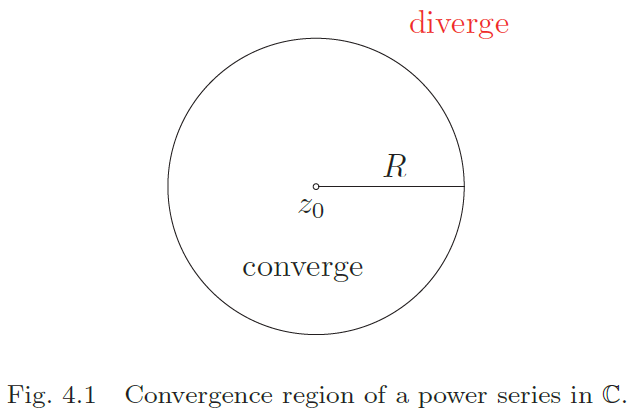
\includegraphics[width=0.5\textwidth]{./SaltChapter/fig-4-1}
\end{center}
\caption{$\mathbb C$에 정의된 제곱급수의 수렴영역}
\label{fig-4-1}
\end{figure}

원 $|z|=R$에서는 어떻게 될까?
복소 제곱급수는 $|z|=R$로 주어진 경계의 모든 점에서 발산하거나,
어떤 점에서는 발산하고 어떤 점에서는 수렴하거나,
아니면 경계의 모든 점에서 수렴할 수도 있다.
경계위의 각 점에 대하여 어떻게 되는지 답을 구하는 일반적인 방법은 없다.
특정한 제곱급수가 주어지면 그 특성에 따라 찾아 직접 확인해야 한다,

{\bf 증명} (정리 \ref{thm-4-1})

\[
S:= \left\{ y\in [0,\infty) \,:\,
\exists z\in \mathbb C, y=|z| \text{ 이고 } \Sum_{n=0}^\infty c_nz^n \text{이 수렴한다.}
\right\}
\]
라 정의하자.
$0\in S$은 분명하기에 $S$는 공집합이 아니며
다음 두 가지 경우가 가능하다.

$\underline{1}^\circ$ $S$가 위로 유계가 아닌 경우:
이 경우는 수렴반경은 무한대가 됨을 보일 것이다.
$z\in \mathbb C$가 주어졌다고 하면,
$|z|<y$인 $y\in S$가 존재한다.
 그런데 $y\in S$이므로 $y=|z_0|$이고
\[
\sum_{n=0}^\infty c_n z_0^n
\]
이 수렴하는 $z_0\in S$가 존재한다.
이로부터 $n\to\infty$일 때 각 항이 $0$으로 수렴한다.
특히, 각 항은  $|c_nz_0^n| \le M$으로 유계이다.
이제 $r:=|z|/|z_0| (<1)$로 잡으면
\[
|c_nz^n| = |c_nz_0^n| \left( \dfrac{|z|}{|z_0|}\right)^n
\le Mr^n \quad (n\in \mathbb N).
\]
한편 $\sum\limits_{n=0}^\infty Mr^n$이 수렴한다 ($r<1$).
비교판정법을 쓰면 
\[
\sum_{n=0}^\infty c_n z^n
\]
은 절대수렴한다. $z$는 우리가 임의로 선택할 수 있기 때문에
정리의 (1)이 성립한다,


$\underline{2}^\circ$ $S$가 위로 유계인 경우:
이 경우 수렴반경이 $\sup S$가 됨을 보일 것이다.
즉,
\begin{itemize}
\item[(a)] $|z|<\sup S$이면
$\Sum_{n=0}^\infty c_nz^n$이 절대수렴하고,
\item[(b)] $|z|>\sup S$이면  $\Sum_{n=0}^\infty c_nz^n$는 발산한다.
\end{itemize}
$z\in S$가 $|z|<\sup S$를 만족하면
상한(supremum)의 %= ##[SALT] 용어확인
정의에 따라,
$|z|<y$인 $y\in S$가 존재한다. 
그러면 $\underline{1}^\circ$ $S$의 증명과정을 아래와 같이 반복할 수 있다.
$y\in S$이므로
$y=|z_0|$이고
\[
\sum_{n=0}^\infty c_n z_0^n
\]
이 수렴하는 $z_0\in S$가 존재한다.
이로부터 $n\to\infty$일 때 각 항이 $0$으로 수렴한다.
특히, 각 항은 $|c_nz_0^n| \le M$으로 유계이다.
이제 $r:=|z|/|z_0| (<1)$로 잡으면
\[
|c_nz^n| = |c_nz_0^n| \left( \dfrac{|z|}{|z_0|}\right)^n
\le Mr^n \quad (n\in \mathbb N).
\]
한편 $\sum\limits_{n=0}^\infty Mr^n$이 수렴한다 ($r<1$).
비교판정법을 쓰면 
\[
\sum_{n=0}^\infty c_n z^n
\]
은 절대수렴한다.
끝으로, $z\in \mathbb C$가 $|z|>\sup S$를 만족하면,
$y:=|z|$라 할 때
$y \in S$이고 $S$의 정의로부터 
\[
\sum_{n=0}^\infty c_n z^n
\]
이 발산한다 (그렇지 않다면 $y\in S$를 만족해야 한다).

\begin{figure*}[h!]
\begin{center}
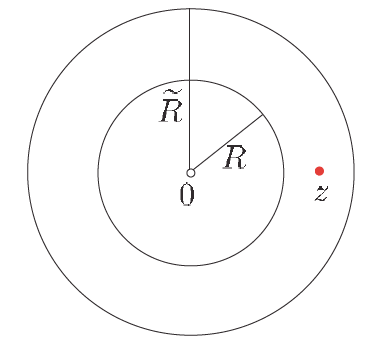
\includegraphics[width=0.3\textwidth]{./SaltChapter/fig-4-0-2}
\end{center}
%\caption{$\mathbb C$에 정의된 제곱급수의 수렴영역}
%\label{fig-4-1}
\end{figure*}

$R$의 유일성은 다음과 같이 증명된다.
$R$과 $\tilde R$이 정리의 조건을 만족하고 $R<\tilde R$이라 하자.
그러면
\[
R < r:= \dfrac{R+\tilde R}{2} < \tilde R.
\]
$r<\tilde R$로부터
$\Sum_{n=0}^\infty c_n r^n$이 수렴하고,
$R<r$로부터 $\Sum_{n=0}^\infty c_n r^n$은 발산하며
모순이 된다.
\hfill $\square$

다음 결과를 이용하면
몇가지 경우의 수렴반경를 계산할 수 있다,

 \begin{salttheorem} {}{} \label{thm-4-2}
제곱급수 
\[
\Sum_{n=0}^\infty c_nz^n
\]에 대하여 극한
$L:= \Lim_{n\to\infty} \left| \dfrac{c_{n+1}}{c_n}\right|$가
존재한다고 하자. 
\begin{itemize}
\item[(1)] $L\ne0$이면, 수렴반경은 $1/L$이고,
\item[(2)] $L=0$이면, 수렴반경은 무한대이다.
\end{itemize}
\end{salttheorem}

{\bf 증명}

$L\ne0$이라 하자.
그러면 $|z|<1/L$인 모든 $z\ne0$에 대하여
$q<1$와 충분히 큰 $N$이 존재하여
\[
\dfrac{|c_{n+1}z^{n+1}|}{|c_nz^n|}
= \left| \dfrac{c_{n+1}}{c_n}\right| |z| \le q <1
\quad (n>N)
\]
을 만족한다
(왜냐하면,
\[
\left|\dfrac{c_{n+1}}{c_n}z\right|
\stackrel{n\to\infty}{\longrightarrow}
L|z|<1
\]
이므로 $q=(L|z|+1)/2 <1$로 잡으면 된다).
비율판정법을 적용하면 급수는 절대수렴한다.

$L=0$이면 $0$이 아닌 모든 $z\in \mathbb C$에 대하여
$q<1$가 존재하여
\[
\dfrac{|c_{n+1}z^{n+1}|}{|c_nz^n|}
= \left| \dfrac{c_{n+1}}{c_n}\right| |z| \le q <1
\quad (n>N)
\]
을 만족한다 (왜냐하면
\[
\left|\dfrac{c_{n+1}}{c_n}z\right|
\stackrel{n\to\infty}{\longrightarrow}
0|z|=0<1
\]
이므로 $q=1/2<1$도 두면된다).
따라서 비율판정법을 다시 쓰면 급수는 절대수렴한다.

한편, $L\ne0$이고 $|z|>1/L$이면,
$\left|\dfrac{c_{n+1}z}{c_n}\right|
\stackrel{n\to\infty}{\longrightarrow}
L|z|>1$이므로
충분히 큰 $N$이 존재하여
\[
\dfrac{|c_{n+1}z^{n+1}|}{|c_nz^n|}
= \left| \dfrac{c_{n+1}}{c_n}\right| |z|>1
\quad (n>N)
\]
을 만족한다.
이 경우 비율판정법에 따라 급수는 발산한다.
\hfill $\square$

\begin{saltexample}[label=example-4-2]{}{}
\[
\lim_{n\to\infty} \dfrac{\dfrac1{(n+1)^2}}{\dfrac1{n^2}} = 1
\]
이므로 
급수 $\Sum_{n=1}^\infty \dfrac{z^n}{n^2}$는
$|z|<1$에서 수렴하고
$|z|>1$에서 발산한다.
$|z|=1$이면
\[
\left| \dfrac{z^n}{n^2} \right| = \dfrac1{n^2}
\]
이므로 급수 $\Sum_{n=1}^\infty \dfrac{1}{n^2}$는
절대수렴한다. 즉, 원 $|z|=1$ 위의 모든 점에서 급수가 수렴한다.
한편 기하급수 
\[
\sum_{n=0}^\infty z^n
\]
은 원 $|z|=1$ 위의 어떤 점에서도 수렴하지 않는다.
\hfill$\diamondsuit$
\end{saltexample}

\begin{salt_exercise}\label{ex-4-6}
급수 $\Sum_{n=0}^\infty c_nz^n$에 대하여
극한 $L:=\Lim_{n\to\infty} \sqrt[n]{|c_n|}$이 존재할 때
다음을 보여라.
\begin{itemize}
\item[(1)] $L\ne 0$이면 수렴반경은 $1/L$이다.
\item[(2)] $L\ne0$이면 수렴반경은 무한대이다.
\end{itemize}
\end{salt_exercise}

\begin{salt_exercise}\label{ex-4-7}
급수 $\Sum_{n=1}^\infty n^nz^n$은
$z=0$에서만 수렴함을 보여라.
\end{salt_exercise}

\begin{salt_exercise}\label{ex-4-8}
급수 $\Sum_{n=1}^\infty \dfrac{z^n}{n^n}$은
모든 $z\in\mathbb C$에 대하여 수렴함을 보여라.
\end{salt_exercise}

\begin{salt_exercise}\label{ex-4-9}
다음 복소제곱급수의 수렴반경을 구하라.
\[
\sum_{n=1}^\infty \dfrac{(-1)^n}{n}z^n,\quad
\sum_{n=0}^\infty n^{2012}z^n, \quad
\sum_{n=0}^\infty \dfrac1{n!}z^n.
\]
\end{salt_exercise}

\subsection{복소해석함수의 제곱급수}

다항식은 수렴반경이 무한대인 제곱급수로 간주할 수 있다.
즉, 모든 $\mathbb C$에서 수렴한다.
이 성질은 복소해석함수에서도 성립하는데
이는 우연이 아니다.
일반적으로 제곱급수 
\[
f(z):= \sum_{n=0}^\infty c_nz^n
\]
가 $|z|<R$에 대하여 수렴하면
$|z|<R$에서 복소해석함수가 되며 
다음 등식이 성립한다.
\[
f'(z) = \dfrac d{dz} (c_0+ c_1z + c_2z^2 + \cdots)
= c_1 + 2c_2z + 3c_3z^3 + \cdots 
= \sum_{n=1}^\infty c_n n z^{n-1}.
\]
(항의 개수가 유한한 경우, 즉, 다항식처럼 
항별 미분이 가능할 것으로 예상한 결과와 같다)

\begin{salttheorem}{}{} \label{thm-4-3}
$R>0$이고 $f(z):= \Sum_{n=0}^\infty c_nz^n$가
$|z|<R$에서 수렴한다고 하면
$f'(z) = \Sum_{n=1}^\infty c_n n z^{n-1}$.
\end{salttheorem}

{\bf 증명}

{\bf 단계 1.}
우선 다음 제곱급수가 $|z|<R$에서 절대수렴함을 보이자.
\[
g(z):= \Sum_{n=1}^\infty c_n n z^{n-1}
=  c_1 + 2c_2z + 3c_3z^3 + \cdots
\]
$z$는 고정하자.
$|z|<r<R$을 만족하는 $r$을 잡으면, 가정으로부터
\[
\Sum_{n=0}^\infty c_nr^n
\]
이 수렴한다. 따라서 모든 $n$에 대하여
$|c_nr^n|<M$을 만족하는 양수 $M$이 존재한다.
$\rho:=|z|/r$이라 하면, $0\le \rho <1$이고,
\[
|nc_nz^{n-1}| = |c_nr^n| \cdot 
\dfrac1r \cdot n \left| \dfrac zr\right|^{n-1}
\le \dfrac{Mn\rho^{n-1}}r.
\]
$\Sum_{n=1}^\infty n\rho^{n-1}$은 
($1/(1-\rho)^2$으로) 수렴한다 (연습문제 \ref{ex-4-4} 참고).
따라서 비교판정법에 의해
$\Sum_{n=1}^\infty nc_nz^{n-1}$은 절대수렴한다.

{\bf 단계 2.}
이제 $|z_0|<R$에 대하여 $f'(z_0) = g(z_0)$임을 보이자. 즉,
\[
\lim_{z\to z_0} \left(
\dfrac{f(z)-f(z_0)}{z-z_0} - g(z_0) \right) = 0.
\]
단계 1에서 했던 것처럼 $|z_0|<r<R$을 만족하는 $r$을 잡으면, 
$z\to z_0$로부터 $|z|<r$도 성립한다.

\begin{figure*}[h!]
\begin{center}
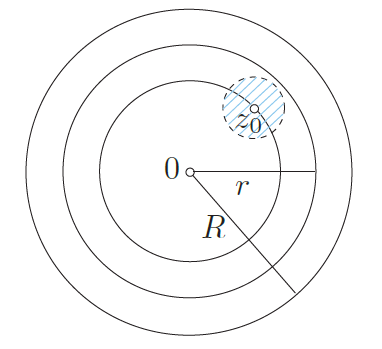
\includegraphics[width=0.3\textwidth]{./SaltChapter/fig-4-0-3}
\end{center}
%\caption{$\mathbb C$에 정의된 제곱급수의 수렴영역}
%\label{fig-4-0-3}
\end{figure*}

$\epsilon>0$이라 하자.
$\Sum_{n=1}^\infty nc_nr^{n-1}$이 절대수렴하므로
다음을 만족하는 $N$이 존재한다.
\[
\Sum_{n=N}^\infty \left| nc_nr^{n-1}\right| < \dfrac \epsilon4.
\]
이제부터 $N$을 고정하자.
$f(z) - f(z_0) = \Sum_{n=1}^\infty c_n(z^n - z_0^n)$이므로,
$z\ne z_0$에 대하여
\[
\dfrac{f(z)-f(z_0)}{z-z_0}  
= \sum_{n=1}^\infty c_n \dfrac{z^n-z_0^n}{z-z_0}
= \sum_{n=1}^\infty c_n \left(
z^{n-1} + z^{n-2}z_0 + \cdots + z_0^{n-1} \right).
\]
따라서,
\[
\dfrac{f(z)-f(z_0)}{z-z_0}   - g(z_0)
= \sum_{n=1}^\infty c_n \dfrac{z^n-z_0^n}{z-z_0}
= \sum_{n=1}^\infty c_n \left(
z^{n-1} + z^{n-2}z_0 + \cdots + z_0^{n-1} - nz_0^{n-1}\right).
\]
이 급수에서 처음 $N-1$개 항의 합을 $S_1$이라 하고
(즉, $n=1$에서 $n=N-1$까지),
$S_2$를 나머지 항의 합이라고 하자.
그러면, $|z|, |z_0| < r$로부터
\[
|S_2| \le \sum_{n=N}^\infty |c_n| 
\left( \underbrace{r^{n-1}+r^{n-1} + \cdots + r^{n-1}}_{n\text{개 항}}
+ nr^{n-1}\right)
= \sum_{n=N}^\infty 2n|c_n|r^{n-1} < \dfrac\epsilon2.
\]
한편,
\[
S_1= \sum_{n=1}^N c_n \left(
z^{n-1} + z^{n-2}z_0 + \cdots + zz_0^{n-2} + z_0^{n-1} - nz_0^{n-1}
\right)
\]
는 $z$의 다항식이며 극한은 다음과 같다.
\begin{align*}
\lim_{z\to z_0} S_1
&= \sum_{n=1}^N c_n \left(
z^{n-1} + z^{n-2}z_0 + \cdots + zz_0^{n-2} + z_0^{n-1} - nz_0^{n-1}
\right) \\
&= \sum_{n=1}^N c_n \left(
nz_0^{n-1}  - nz_0^{n-1} \right) = 0.
\end{align*}
따라서
$|z-z_0|<\delta$이면, $|S_1|< \epsilon/2$가 되는 
양수 $\delta$가 존재한다.
이제 $|z|<r$이고 $0<|z-z_0|< \delta$에 대하여
\[
\left| \dfrac{f(z)-f(z_0)}{z-z_0}   - g(z_0) \right|
\le |S_1| + |S_2| <  \dfrac\epsilon2 + \dfrac\epsilon2 = \epsilon.
\]
이로써 $f'(z_0) = g(z_0)$가 증명된다.
\hfill $\square$

\begin{salt_remark} \label{rem-4-1}
$(c_n)_{n\in\mathbb N}$이 실수열일 때,
실제곱급수
\[
\sum_{n=0}^\infty c_nx^n
\]
\end{salt_remark}
를 생각해보자. 실해석의 결과로부터 어떤 $R>0$이 존재하여
이 제곱급수는 구간 $(-R, R)$에서 수렴하고
$\mathbb R \setminus [-R,R]$에서 발산한다.
정리 \ref{thm-4-1}과 \ref{thm-4-3}로부터
실변수 $x$를 복소변수 $z$로 바꾸면 실제곱급수의 결과가 
복소평면의 원판 $|z|<R$에 정의된 복소해석함수로 확장됨을 알 수 있다.
따라서
실해석함수(즉, 국소적으로 제곱급수 전개를 갖는 실변수함수)는
복소해석함수를 실수축에 제한한 것으로 볼 수 있다.
이 결과로 실해석학과 복소해석학의 세계를 연결하는
상호작용을 엿볼 수 있다
(우리는 코시-리만 방정식을 공부하면서 이미 이러한 사례를 살펴 본 바 있다).

앞의 결과를 반복하면 다음을 쉽게 얻는다.

\begin{salt_corollary}\label{coro-4-1}
$R>0$이고, $f(z):= \Sum_{n=0}^\infty c_n z^n$이 $|z|<R$에서 수렴한다고 하자.
그러면, $k\ge1$에 대하여
\begin{equation}\label{eq-4-1}
f^{(k)}(z) = \sum_{n=k}^\infty n(n-1)(n-2)\cdots (n-k+1)c_nz^{n-k}.
\quad (|z|<R)
\end{equation}
특히, $n\ge0$에 대하여, $c_n = \dfrac1{n!} f^{(n)}(0)$.
\end{salt_corollary}

{\bf 증명}

직접 계산하여 바로 얻을 수 있는 결과이며, 두번째 결과를 얻기 위해
식 \eqref{eq-4-1}에 $z=0$을 대입하면
\[
f^{(k)}(0) = k(k-1)\cdots 1c_k + z \sum{n=k+1}^\infty n(n-1) \cdots (n-k+1)c_n z^{n-k-1}\Big|_{z=0}
= k!c_k
\]
이며, $f(0)=c_0$이다.
\hfill $\square$

이는 $0$을 중심으로 전개한 제곱급수에 한정된 결과가 아니다.
복소수 $z_0$를 택하여 제곱급수
\[
\sum_{n=0}^\infty c_n(z-z_0)^n
\]
를 생각하면, 정리 \ref{thm-4-1}과 \ref{thm-4-3}으로부터
다음 결과를 바로 얻는다.


\begin{salt_corollary} \label{thm-4-2}
제곱급수 $\Sum_{n=0}^\infty c_n(z-z_0)^n$에 대하여
다음 두 가지 중 정확히 하나만 성립한다.
\begin{itemize}
\item[(1)] 모든 $z\in\mathbb C$에 대하여 절대수렴하거나
\item[(2)] 음이 아닌 실수 $R$이 유일하게 존재하여 다음을 만족한다.
\begin{itemize}
\item[(a)] $|z-z_0|<R$인 모든 $z\in\mathbb C$에 대하여 
$\Sum_{n=0}^\infty c_n(z-z_0)^n$이 절대수렴하고,
\item[(b)] $|z-z_0|>R$인 모든 $z\in\mathbb C$에 대하여 
$\Sum_{n=0}^\infty c_n(z-z_0)^n$는 발산한다.
\end{itemize}
\end{itemize}
\end{salt_corollary}

\begin{salt_corollary}\label{coro-4-3}
$z_0\in \mathbb C$, $R>0$이고, 
$f(z):= \Sum_{n=0}^\infty c_n (z-z_0)^n$이 $|z-z_0|<R$에서 수렴한다고 하자.
그러면, $k\ge1$에 대하여
\[
f^{(k)}(z) = \sum_{n=k}^\infty n(n-1)(n-2)\cdots (n-k+1)c_n(z-z_0)^{n-k}.
\quad (|z-z_0|<R)
\]
특히, $n\ge0$에 대하여, $c_n = \dfrac1{n!} f^{(n)}(z_0)$.
\end{salt_corollary}

\begin{salt_remark} [계수의 유일성] \label{rem-4-2}
중심이 $z_0$, 반지름 $R>0$인 열린원판에서
두 제곱급수
\[
\Sum_{n=0}^\infty c_n(z-z_0)^n \quad\text{와}\quad
\Sum_{n=0}^\infty \tilde c_n(z-z_0)^n
\]
가 모두 같은 함수 $f$로 수렴한다고 하자.
그러면 위의 따름정리로부터 모든 $n\ge0$에 대하여
\[
c_n = \dfrac{f^{(n)}(z_0)}{n!} = \tilde c_n.
\]
\end{salt_remark}

\begin{salt_exercise} \label{ex-4-10}
$|z|<1$일 때,
$1^2 + 2^2z + 3^2z^2 + 4^2z^3 + \cdots$의 값은?
\end{salt_exercise}

\begin{salt_exercise} \label{ex-4-11}
제곱급수 $\Sum_{n=0}^\infty c_nz^n$에 대하여 다음 문장의 참, 거짓을 판정하라.
\begin{itemize}
\item[(1)] 급수가 수렴하는  복소수 $z$의 집합은 $\{0\}$이거나, 유한한 반지름을 갖는 열린원판,
또는 복소평면 전체가 되며 다른 경우는 생길 수 없다.
\item[(2)] 제곱급수가 $z=1$에서 수렴하면 $|z|<1$에서 수렴한다.
\item[(3)] 제곱급수가 $z=1$에서 수렴하면 원 $|z|=1$의 모든 점에서 수렴한다.
\item[(4)] 제곱급수가 $z=1$에서 수렴하면 $z=-1$에서 수렴한다.
\item[(5)] 제곱급수가 원점이 중심이고 반지름이 유한한 열린원판에서 수렴하면
원판의 경계(즉, 원판을 둘러싸는 원)의 전체 또는 일부에서도 수렴할 수 있으나
그 이외의 점에서는 수렴할 수 없다.
\item[(6)] 수렴하는 범위가 닫힌원판 $|z|\le 1$ 전체인 제곱급수가 존재한다.
\item[(7)] 제곱급수가 $z=i$에서 발산하면, $z=1+i$에서도 발산한다.
\end{itemize}
\end{salt_exercise}

\section{테일러 급수} \label{section-4-3}

앞 절에서 수렴반경이 $R$인 복수제곱급수
\[
\sum_{n=0}^\infty c_n(z-z_0)^n
\]
은 영역 $|z-z_0|<R$에서 복소해석함수가 됨을 살펴보았다.
이 절에서는 역으로 $f$가 원판 $|z-z_0|<R$에서 복소해석함수이면
\[
f(z) = \sum_{n=0}^\infty c_n (z-z_0)^n \quad (|z-z_0|<R)
\]
임을 보일 것이다. 여기서 계수 $c_n$은 $f$로부터 결정된다.
따라서 영역 $D$에 정의된 복소해석함수 $f$는 임의의 점 $z_0\in D$의 근방에서
제곱급수 전개를 갖는다.

\begin{salttheorem} {}{} \label{thm-4-4}
$f$가 $D(z_0,R) := \{ z\in \mathbb C \,:\, |z-z_0| <R \}$에서 복소해석함수이면,
$z\in D(z_0,R)$에 대하여
$f(z) = c_0 + c_1(z-z_0) + c_2(z-z_0)^2 + c_3(z-z_0)^3+ \cdots$이다.
여기서, $n\ge0$에 대하여
\[
c_n = \dfrac1{2\pi i} \int_C \dfrac{f(\zeta)}{(\zeta-z_0)^{n+1}} d\zeta
\]
이고, $C$는 중심이 $z_0$이고 반지름 $r$ ($0<r<R$)인 원을 반시계방향으로 도는 원이다.
\end{salttheorem}

\begin{figure*}[h!]
\begin{center}
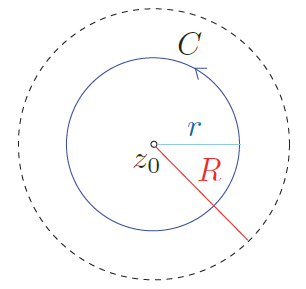
\includegraphics[width=0.3\textwidth]{./SaltChapter/fig-4-0-4}
\end{center}
%\caption{$\mathbb C$에 정의된 제곱급수의 수렴영역}
%\label{fig-4-0-3}
\end{figure*}

{\bf 증명}

$z\in D(z_0, R)$이라 하자.
우선 $|z-z_0|<r<R$인 $r$을 잡고
코시 적분공식을 적용하면
\begin{align*}
f(z) &= \dfrac1{2\pi i}\int_C \dfrac{f(\zeta)}{\zeta-z} d\zeta
= \dfrac1{2\pi i}\int_C \dfrac{f(\zeta)}{\zeta-z_0+z_0-z} d\zeta \\
&= \dfrac1{2\pi i}\int_C \dfrac{f(\zeta)}{(\zeta-z_0)\left(1- \dfrac{z-z_0}{\zeta-z_0}\right)} d\zeta.
\end{align*}
$w:=\dfrac{z-z_0}{\zeta-z_0}$라 하면,
$|w| = \dfrac{|z-z_0|}r <1$이므로
\begin{align*}
\dfrac1{1-\dfrac{z-z_0}{\zeta-z_0}} = \dfrac1{1-w}
& = 1+ w + w^2 + w^3 + \cdots + w^{n-1} + \dfrac{w^n}{1-w} \\
&= 1 + \dfrac{z-z_0}{\zeta-z_0} + \cdots + \dfrac{(z-z_0)^{n-1}}{(\zeta-z_0)^{n-1}}
+ \dfrac{(z-z_0)^n}{(\zeta-z_0)^{n-1}(\zeta-z)}.
\end{align*}
이 결과를 종합하면
\begin{align*}
f(z) &= \dfrac1{2\pi i}\int_C f(\zeta) \left(
\dfrac1{\zeta-z_0} + \cdots + \dfrac{(z-z_0)^{n-1}}{(\zeta-z_0)^{n}}
+ \dfrac{(z-z_0)^n}{(\zeta-z_0)^{n}(\zeta-z)} \right) d\zeta \\
&= c_0 + c_1(z-z_0) + \cdots + c_{n-1}(z-z_0)^{n-1} + R_n(z),
\end{align*}
여기서 
\[
R_n(z) := \dfrac1{2\pi i} \int_C \dfrac{f(\zeta)(z-z_0)^n}{(\zeta-z_0)^n(\zeta-z)}d\zeta.
\]
이제 $n\to\infty$일 때, $R_n(z)$가 $0$으로 수렴하는 것을 보이면 증명이 끝난다.
콤팩트 집합의 연속 실함수이므로 $|f|$는 원 위에서 유계이다.
즉, 원 위의 모든 $\zeta\in C$에 대하여 $|f(\zeta)|<M$을 만족하는 상수 $M>0$이 존재한다
(약간 왜곡하면 경로 $C$를 생각할 때, 점 $C(t)$의 집합 ($t\in [0,2\pi]$)으로 간주할 수 있다).
또한 $\zeta\in C$에 대하여
\[
\left| \dfrac{(z-z_0)^n}{(\zeta-z_0)^n}\right| 
= \left( \dfrac{|z-z_0|}r \right)^n
\stackrel{n\to\infty}{\longrightarrow} 0.
\]
한편 $\zeta\in C$에 대하여 $1/|\zeta-z|$는 어떻게 되는가?
어떤 수로 유계임을 보일 수 있는가?
아래 그림을 보면 실제로 원 $C$와  $z$의 거리의 역수로 유계이다.

\begin{figure*}[h!]
\begin{center}
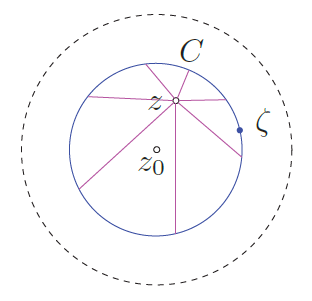
\includegraphics[width=0.3\textwidth]{./SaltChapter/fig-4-0-5}
\end{center}
%\caption{$\mathbb C$에 정의된 제곱급수의 수렴영역}
%\label{fig-4-0-3}
\end{figure*}

$|\zeta-z| = |\zeta-z_0-(z-z_0)| \ge
|\zeta-z_0| - |z-z_0| = r - |z-z_0|$이므로
\[
|R_n(z)| \le \left( \dfrac{|z-z_0|}r \right)^n \dfrac M{r-|z-z_0|} 
\stackrel{n\to\infty}{\longrightarrow} 0.
\]
따라서 제곱급수 $c_0 + c_1(z-z_0) + c_2(z-z_0)^2 + c_3(z-z_0)^3+ \cdots$는
$f(z)$로 수렴한다.
지금까지 결과로
\[
c_n = \dfrac1{2\pi i} \int_C \dfrac{f(\zeta)}{(\zeta-z_0)^{n+1}} d\zeta
\]
이 $|z-z_0|<r<R$인 $r$에서 성립한다는 것만을 보였다.
하지만 코시 적분정리를 사용하면 적분이 $r$에 무관함을 알 수 있고
$r\in (0,R)$이 다음을 만족하도록 선택할 수 있다.
\begin{itemize}
\item[(1)] $\dfrac{f(\cdot)}{(\cdot - z_0)^{n+1}}$이 
$0<|z-z_0|<R$인 뚫린 원판 $D_*(z_0,R)$에서 복소해석함수이다.
\item[(2)] $C$이외의 다른 경로로 중심이 $z_0$, 반지름 $\tilde r\in (0,R)$인 원 $\tilde C$를 잡으면
$C$와 $\tilde C$는 $D_*(z_0,R)$에서 호모토픽하다. 
\end{itemize}
이로써 증명이 완성된다. \hfill $\square$

한편 정리 \ref{thm-4-3}으로부터
\[
f(z) = \sum_{n=0}^\infty c_n(z-z_0)^n
\quad (|z-z_0| <R)
\]
로 정의하면 $n\ge0$에 대하여 $c_n = \dfrac{f^{(n)}(z_0)}{n!}$이다.
이상에서 적분으로 주어진 계수 $c_n$에 대한  다른 표현식을 얻었다.
하지만 임의의 원판에서 제곱급수를 전개할 때 계수는 유일하게 결정된다.
따라서 두 표현식은 같은 결과가 된다는 것을 기억하면 다음 결과를 얻는다.

\begin{salt_corollary}(테일러\footnote{
이 급수 전개에 대하여 연구한 학자 중 실해석 함수 관점에서 연구한
브룩 테일러(Brook Taylor, 1685-1731)의 이름이다.
}
 급수) \label{coro-4-4}
\begin{itemize}
\item[(1)] $D$가 영역이고,
\item[(2)] $f:D\to \mathbb C$가 복소해석함수이고,
\item[(3)] $z_0\in D$ 이면,
\end{itemize}
\[
f(z) = f(z_0) + \dfrac{f'(z_0)}{1!}(z-z_0) + \dfrac{f''(z_0)}{2!}(z-z_0)^ 2 
+ \cdots, \quad |z-z_0|<R.
\]
여기서 $R$은 $z_0$를 중심으로 하는 원판 중 영역 $D$에 속하는 가장 큰 열린집합의
반지름이다. 또한,
\begin{equation} \label{eq-4-2}
f^{(n)}(z_0) = \dfrac{n!}{2\pi i}\int_C \dfrac{f(z)}{(z-z_0)^{n+1}}dz.
\end{equation}
\end{salt_corollary}
단, $C$는 $z_0$를 중심으로 하는 반지름 $r$ ($0<r<R$)인 원을 반시계방향으로 회전하는 경로이다.

식 \eqref{eq-4-2}는 (일반화된) 코시 적분공식이라 불린다. 우리는 앞서 $n=0$인 경우(정리 \ref{thm-3-4})와
$n=1$인 경우(정리 \ref{thm-3-6}의 증명)에 대하여 증명했었다.
여기에 더하여 위 결과로부터 임의의 점 $w\in \Delta:=\{z\in\mathbb C\,:\, |z-z_0| <R \}$에 
대하여 다음 식을 얻는다.
\[
f^{(n)}(w) = \dfrac{n!}{2\pi i}\int_C \dfrac{f(z)}{(z-w)^{n+1}}dz.
\]
이는 코시 적분정리로부터 얻어지는데,
우선 $w$를 중심으로 하는 작은 원 $C_\delta$에 대하여 위 식을 증명한 다음
경로 $C$와 $C_\delta$가 $\Delta\setminus \{w\}$-호모토픽이며,
$f(\cdot)/(\cdot-w)^{n+1}$이 $\Delta\setminus \{w\}$에서 복소해석함수임을 이용하여 보일 수 있다.

{\bf 증명}

정리 \ref{thm-4-4}로부터,
중심이 $z_0$이고 $D(z_0,R):= \{ z\in \mathbb C \,:\, |z-z_0|<R\}$가
$D$에 포함되는 가장 큰 열린원판이 되도록 $R$을 선택한다.
\begin{equation}\label{eq-4-3}
f(z) = c_0 + c_1(z-z_0) + c_2(z-z_0)^2 + c_3(z-z_0)^3 + \cdots, \quad
z\in D(z_0,R).
\end{equation}
또한, $n\ge0$에 대하여
\[
c_n = \dfrac1{2\pi i} \int_C \dfrac{f(z)}{(z-z_0)^{n+1}} dz,
\]
여기서 $C$는 $z_0$를 중심으로 하는 반지름 $r$ ($0<r<R$)인 원을 반시계방향으로 회전하는 경로이다.
한편, 따름정리 \ref{coro-4-3}에 의하여
제곱급수는 무한번 미분가능하고, $n\ge0$에 대하여
\[
\dfrac1{n!}f^{(n)}(z_0) = c_n
\]
이므로 원하는 결과를 얻는다. \hfill $\square$

요약하면, 
$f$가 영역 $|z-z_0|<R$에 정의된 복소해석함수이면, $|z-z_0|<R$에서
\[
f(z) = \sum_{n=0}^\infty \left( \dfrac 1{2\pi i}
\int_C \dfrac{f(\zeta)}{(\zeta - z_0)^{n+1}}d\zeta \right)\cdot
(z-z_0)^n
=  \sum_{n=0}^\infty \dfrac{f^{(n)}(z_0)}{n!} (z-z_0)^n,
\]
여기서 $C(t) = z_0 + r\exp (it)$ ($t\in[0,2\pi]$)이고 $r$은
$0<r<R$을 만족하는 임의의 실수이다.

\begin{saltexample}[label=exxample-4-3]{}{}
지수함수 $f$, $z\mapsto f(z):=\exp z$는 전해석함수이다.
따라서 적당한 계수 $c_n$에 대하여
\[
\exp z = \sum_{n=0}^\infty c_nz^n \quad (z\in \mathbb C)
\]
로 쓸 수 있다. 
다음 식으로 주어진 계수들을 실제로 구하면?
\[
c_n = \dfrac1{n!}f^{(n)}(z_0), \quad n\ge 0
\]
$\dfrac d{dz}\exp z = \exp z$이고$f^{(n)}(0)=1$이므로
\[
f(z) = \sum_{n=0}^\infty \dfrac{f^{(n)}(0)}{n!} (z-0)^n 
=\sum_{n=0}^\infty \dfrac{1}{n!} z^n\quad (z\in\mathbb C).
\]
\hfill $\diamondsuit$
\end{saltexample}

\begin{saltexample}[label=exxample-4-4]{}{}
$f(z) = \Log(z)$로 정의된 함수 $f$는 $\mathbb C\setminus (-\infty,0]$에서 
복소해석함수이다. 이 잘린 평면에서 $z_0=1$을 중심으로 가장 큰 열린원판을 잡으면
$D = \{z\in\mathbb C\,:\, |z-1|<1\}$이다.
\[
f^{(n)}(z_0) = \dfrac{(-1)^n(n-1)!}{z_0^n} = (-1)^n (n-1)!
\]
이므로 $|w|<1$에 대하여
\[
\Log (1+w) = w - \dfrac {w^2}{2} + \cdots + \dfrac{(-1)^nw^n}n + \cdots
\]
를 얻는다. \hfill $\diamondsuit$
\end{saltexample}

\begin{salt_exercise} \label{ex-4-12}
$z\in\mathbb C$에 대하여 다음 등식을 보여라.
\[
\sin z = z - \dfrac{z^3}{3!} + \dfrac{z^5}{5!} - \cdots,
\quad
\cos z = 1 - \dfrac{z^2}{2!} + \dfrac{z^4}{4!} - \cdots.
\]
\end{salt_exercise}

\begin{salt_exercise} \label{ex-4-13}
$z_0=1$을 중심으로 하여
다항식 $z^6-z^4 + z^2 -1$의 테일러 급수를 구하라.
\end{salt_exercise}

\begin{salt_exercise} \label{ex-4-14}
함수 $f$가 다음과 같을 때 테일러 급수 $\Sum_{n=0}^\infty c_nz^n$의 계수 $c_n$을 구하라.
\begin{itemize}
\item[(1)] $f(z) = \dint_{\gamma_{0z}} \exp(\zeta^2)d\zeta$ ($z\in\mathbb C$),
단, $\gamma_{0z}$는 $0$에서 $z$까지 연결하는 직선 경로이다. \\
힌트: $f'(z) = \exp(z^2)$.
\item[(2)] $f(z) = \dfrac{z^2}{(z+1)^2}$ ($z\in \mathbb C\setminus \{-1\}$). \\
힌트: $|z|<1$에 대하여, $\dfrac1{z+1} = 1- z + z^2 - \cdots$.
\end{itemize}
\end{salt_exercise}

일반화된 코시 적분정리에서 얻어지는 결과를 더 살펴보자.

\begin{salt_corollary}[코시 부등식] \label{coro-4-5}
\ 
\begin{itemize}
\item[(1)] $f$가 $D(z_0, R):= \{z \in \mathbb C\,:\, |z-z_0| <R \}$에 정의된
복소해석함수이고,
\item[(2)] 모든 $z\in D(z_0,R)$에 대하여 $|f(z)|\le M$이면,
\end{itemize}
$n\ge0$에 대하여  \ $|f^{(n)}(z_0)| \le \dfrac{n! M}{R^n}$.
\end{salt_corollary}

{\bf 증명}

$C$가 $z_0$를 중심으로 하고 반지름이 $r<R$인 원이라 하자. 그러면
\begin{align*}
|f^{(n)}(z_0)| &= \left| \dfrac{n!}{2\pi i} \int_C \dfrac{f(z)}{(z-z_0)^{n+1}}dz \right| \\
&\le \dfrac{n!}{2\pi} \max_{z\in C} \left| \dfrac{f(z)}{(z-z_0)^{n+1}} \right| \cdot 
2\pi r = \dfrac{n!}{2\pi} \dfrac{M}{r^{n+1}}2\pi r = \dfrac{n! M}{r^n}.
\end{align*}
극한 $r\nearrow R$을 취하면 원하는 결과를 얻는다. 
\hfill $\square$

\begin{salt_exercise} \label{ex-4-15}
$f$가 전해석함수이고 모든 $z\in\mathbb C$에 대하여
$|f(z)| \le M|z|^n$을 만족하는  $M>0$과 정수 $n\ge0$가 존재한다고 가정하자.
코시 부등식을 이용하여 모든 $z$에 대하여 $f^{(n+1)}(z) = 0$을 증명하고
$f$는 $n$차 이하 다항식임을 보여라. $n=0$일 때는 어떤 결론을 얻는가?
\end{salt_exercise}

\begin{salt_exercise} \label{ex-4-16}
$C$가 원점을 중심으로 반지름 $1$인 원을 반시계방향으로 도는 원형 경로일 때,
$\dint_C \dfrac{\sin z}{z^{2013}}dz$를 구하라.
\end{salt_exercise}

\section{근의 분류}

영역 $D$에서  $f: D\to \mathbb C$가 복소해석함수라고 하자.
항등적으로 $0$이 아닌 함수 $f$의 근은 어떤 모습일까?
($f(z_0)=0$를 만족하는 점 $z_0\in D$를 $f$의 {\bf 근(zero)}이라 한다)
이 절에서는 이 문제의 답으로 근들이 ``고립''되어 있음을 보일 것이다.
연속함수의 경우는 이러한 일이 일어나지 않는다. 
연속함수는 복소해석함수만큼 엄격한 조건을 갖지 않기 때문에
의 근이 고립될 필요가 없다.

\begin{saltexample}[label=example-4-5]{}{}
\begin{itemize}
\item[(1)] $\exp z$는 $\mathbb C$에서 근을 갖지 않는다.
실제로, 모든 $z\in \mathbb C$에 대하여 $|\exp(z)| = e^{\Re(z)} >0$이다.
\item[(2)] $\cos z - 3$은 $\mathbb C$에서 무한이 많은 근 
$2\pi n \pm i \log(3+2\sqrt{2})$ ($n\in\mathbb Z$)
을 갖는다.
모든 근은 수평선에 분포하고 인접한 근과의 간격은 $2\pi$이다.
계산방법은 연습문제 \ref{ex-1-38}을 참고하라.
\item[(3)] 다항식 $p(z) = (z+1)^3z^9(z-1)^9$은 $-1, 0, 1$에서 근을 갖는다. 
\hfill $\diamondsuit$
\end{itemize}
\end{saltexample}

$p$가 항등적으로 $0$이 아닌 다항식이고 $p(z_0)=0$이면
나눗셈정리에 따라 
\[
p(z) = (z-z_0) q(z)
\]
을 만족하는 다항식 $q$(몫)가 존재한다
(즉, 나머지가 $0$이다). 
이제 다음 두 가지  가능성을 생각할 수 있다.
\begin{itemize}
\item[$1^\circ$] $q(z_0) \ne0$. 그러면 $z_0$는 $p$의 고립 근이다.
\item[$2^\circ$] $q(z_0) =0$. 그러면 $p$를 $q$로 바꾸어 위 과정을 반복한다.
\end{itemize}

궁극적으로 적당한 $m\ge1$에 대하여 $p(z) = (z-z_0)^mq(z)$이고  $q(z_0)\ne0$에 도달한다.
이 때 $m$을 ($p$의 근) $z_0$의 중복도(multiplicity) 또는 차수(order)라 부른다.
아래 명제 \ref{prop-4-1}에서 복소해석함수 $f$에서도 (다항식 $p$를 대체하여)
같은 종류의 결과를 얻을 수 있음을 보일 것이다.
다만, 결과가 다항식 $q$ 대신 복소해석함수 $g$로 마무리된다는 것만 다르다.
이는 아주 놀라운 결과는 아니다. 왜냐하면, 제곱급수는 다항식으로부터 유추될 수 있고
임의의 복소해석함수는 국소적으로 제곱급수 전개가 가능하기 때문이다.
우선 다음 정의를 만들자.

\begin{saltdefinition}{}{} \label{def-4-2}
$D$가 영역이고, $f:D\to\mathbb C$가 $D$에서 복소해석함수라고 하자.
$f(z_0)=0$이면 점 $z_0\in D$를 $f$의 {\bf 근}이라고 한다.
다음 조건을 만족하는 가장 작은 자연수를 $m\in\mathbb N$이 존재하면,
\begin{itemize}
\item[(1)] $f^{(m)}(z_0) \ne 0$이고,
\item[(2)] $f(z_0) = \cdots = f^{(m-1)}(z_0) = 0$.
\end{itemize}
$z_0$는 $f$의 {\bf $m$ 중근}이라 한다
(관습적으로 $f^{(0)} := f$라 한다).
\end{saltdefinition}

그러면, 복소해석함수의 근의 분류에 대한 다음 결과를 얻는다.

\begin{saltprop} [근의 분류]{}{} \label{prop-4-1}
\begin{itemize}
\item[(1)] $D$가 영역이고,
\item[(2)] $f:D\to\mathbb C$가 $D$에서 복소해석함수이고,
\item[(3)] $z_0 \in D$가 $f$의 근이라고 하자.
\end{itemize}
그러면, 정확히 다음 두 가지 가능성이 있다.
\begin{itemize}
\item[$1^\circ$] 양수 $R$이 존재하여 $|z-z_0|<R$인 모든 $z$에 대하여
$f(z)=0$.
\item[$2^\circ$] $m\in\mathbb N$이 존재하여
 $z_0$가 $f$의 $m$중근이다. 또한, 
 $g(z_0)\ne0$이고 모든 $z\in D$에 대하여 $f(z) = (z-z_0)^mg(z)$인
 복소해석함수 $g:D\to\mathbb C$가 존재한다.
\end{itemize}
\end{saltprop}

$2^\circ$의 경우 $g$가 연속이고 $g(z_0)\ne0$이므로
$g$는 $z_0$를 중심으로 하는 작은 원판 $\Delta$에서 $0$이 아니며,
$z\in \Delta\setminus \{z_0\}$에서 $f(z) = (z-z_0)^mg(z) \ne 0$이므로
$f$는 $\Delta\setminus \{z_0\}$에서 $0$이 아니다.
따라서 $z_0$는 $\Delta$에서 $f$ 의 유일한 근이다. 즉, 고립된 근이다.

한편, 앞으로 보게 될 항등정리에 따르면
$1^\circ$의 경우는 영역 $D$ 전체에서 $f\equiv 0$이다.

{\bf 증명}

중심이 $z_0$이고 반지름 $R>0$인 원판에서 $f$의 제곱급수 전개를 하면,
\[
f(z) = c_0 + c_1(z-z_0) + c_2(z-z_0)^2 + c_3(z-z_0)^3 + \cdots, \quad
(|z-z_0| <R).
\]
$f(z_0)=0$이므로, $c_0=0$임을 바로 알 수 있다. 
이제 정확히 두 가지 가능성이 있다.
\begin{itemize}
\item[$1^\circ$] 모든 $c_n$이 $0$이다. 그러면, $|z-z_0| <R$에서 $f(z)=0$이다.
\item[$2^\circ$] $c_m\ne 0$인 가장 작은 $m\ge1$이 존재한다.
그러면 $c_0=c_1=\cdots = c_{m-1}=0$이고,
\[
c_n = \dfrac{f^{(n)}(z_0)}{n!}, \quad n\ge0
\]
로부터 $z_0$는 $m$ 중근이다.
또한, 제곱급수 전개로부터 $|z-z_0|<R$에 대하여
\begin{equation} \label{eq-4-4}
f(z) = c_m(z-z_0)^m + c_{m+1}(z-z_0)^{m+1} + \cdots
= (z-z_0)^m \sum_{k=0}^\infty c_{m+k} (z-z_0)^k.
\end{equation}
따라서 $g:D\to \mathbb C$를 
\[
g(z) = \begin{cases}
\dfrac{f(z)}{(z-z_0)^m}, & z\ne z_0, \\
\Sum_{k=0}^\infty c_{m+k} (z-z_0)^k, & |z-z_0|<R
\end{cases}	
\]
로 정의하면,
식 \eqref{eq-4-4}로부터 두 가지 조건을 모두 만족하는 경우
두 가지 경우의 계산결과가 일치하므로
$g$는 잘 정의된다. 추가적으로 다음 결론을 얻는다.
\begin{itemize}
\item[(1)]  $g$는 $D$에서 복소해석함수이다. $z\ne z_0$에서
$f$와 $1/(\cdot - z_0)^m$이 $D\setminus \{z_0\}$에서 복소해석함수이므로
$|z-z_0|<R$에 대하여 제곱급수로 정의된 $g$는 복소해석함수이다.
\item[(2)] $g(z_0) = c_m\ne 0$ ($m$의 정의에서)
\item[(3)] 식 \eqref{eq-4-4}로부터 $z\in D\setminus \{z_0\}$에 대하여
$f(z) = (z-z_0)^mg(z)$. 한편, $z=z_0$이면 양변이 $0$이 된다.
따라서 모든 $z\in D$에 대하여 $f(z) = (z-z_0)^mg(z)$이 성립한다.
\item[(4)] $z_0$는 $m$ 중근이다.
왜냐하면, 모든 $n$에 대하여 $c_n = f^{(n)}(z_0)/n!$이므로
$c_m \ne 0$이고, $c_0 = c_1 = \cdots = c_{m-1}= 0$.
\end{itemize}
\end{itemize}
이상에서 정리가 증명된다. \hfill $\square$

\begin{saltexample}[label=example-4-6]{}{}
\begin{itemize}
\item[(1)] $n\in \mathbb Z$에 대하여 $n\pi$는 $\sin z$의 근이다.
$\sin z$를 실수축에 한정하면 $n\pi$의 근방에서 
$\sin z$가 항등적으로 $0$이 아님을 알 수 있다.
$\sin z$의 근으로서 $n\pi$는 몇 중근인가?
$\sin `z = \cos z$이고, $\cos z \Big|_{z=n\pi}= (-1)^n \ne 0$이므로
$n\pi$는 $\sin z$의 근이지만 중근이 아니다.
\item[(2)] $\exp(0^2) -1 = 1-1 = 0$이므로
$\exp (z^2) -1$은 근으로 $0$을 갖는다.
몇 중근일까?
\[
\exp (z^2) = 1 + \dfrac{z^2}{1!} + \dfrac{z^4}{3!} + \cdots,
\quad z\in \mathbb C
\]
이고, $\exp(z^2) -1 = z^2g(z)$ ($z\in \mathbb C$),
여기서 $g(z):= \dfrac1{1!} + \dfrac{z^2}{2!} = \cdots$.
$g$는 $\mathbb C$에서 수렴하는  제곱급수로 전개되므로
전해석함수이다. 또한, $g(0)=1\ne 0$이다.
따라서 $0$은 $\exp(z^2) -1$의 2중근이다.
다른 방법으로 보일 수도 있다.
\begin{align*}
\dfrac{d}{dz} (\exp(z^2)-1) \Big|_{z=0} 
&= (\exp(z^2))\cdot 2z  \Big|_{z=0}  = 0, \\
\dfrac{d^2}{dz^2} (\exp(z^2)-1)\Big|_{z=0} 
&=  (\exp(z^2))\cdot 2 \Big|_{z=0}  +  (\exp(z^2))\cdot (2z^2)  \Big|_{z=0}  \\
&= 2\ne 0.
\end{align*}
$\exp(z^2) -1$의 근으로서 $0$은 이중근이다.
\end{itemize}
\end{saltexample}

\begin{salt_exercise} \label{ex-4-17}
$D$가 영역이고, $m\in \mathbb N$, $R>0$, $z_0\in D$라고 하자.
복소해석함수 $f,g: D\to \mathbb C$가 $g(z_0)\ne0$이고
$|z-z_0|<R$에 대하여 $f(z) = (z-z_0)^m g(z)$이면,
$z_0$가 $f$의 $m$ 중근임을 증명하라.
\end{salt_exercise}

\begin{salt_exercise} \label{ex-4-18}
함수 $f$를 다음과 같이 정의할 때 $f$의 근 $z_0$의 차수는?
\begin{itemize}
\item[(1)]  $z_0 = i$, $f(z) = (1+z^2)^4$.
\item[(2)]  $z_0 = 2n\pi i$ ($n$은 정수), $f(z) = \exp z -1$.
\item[(3)] $z_0=0$, $f(z) = \cos z - 1 + \dfrac12(\sin z)^2$.
\end{itemize}
\end{salt_exercise}

\begin{salt_exercise} \label{ex-4-19}
$f$가 원 $\gamma$를 내부에 포함하는 원판에서 복소해석함수라고 하자.
원판 내부에서 $f$의 유일한 근 $z_0$의 차수는 1이고,
$z_0$는 원 $\gamma$의 내부에 있다.
다음을 증명하라.
\[
z_0 = \dfrac1{2\pi i} \int_\gamma \dfrac{zf'(z)}{f(z)} dz.
\]
\end{salt_exercise}

\begin{salt_exercise} \label{ex-4-20}
$f$가 영역 $D$에서 복소해석함수이고 $z_0\in D$에서
차수 $m$의 근을 갖는다고 하자.
함수 $z \mapsto (f(z))^2$은 차수 $2m$의 근을 가지며,
$f'$은 차수 $m-1$의 근을 가짐을 보여라.
\end{salt_exercise}

\begin{salt_exercise} \label{ex-4-21}
복소 연속함수의 경우는 명제 \ref{prop-4-1}의 복소해석함수에 대한
이분법적 결론을 적용할 수 없다. 
$f:\mathbb C \to \mathbb C$에 대하여 
$0$이  고립된 근도 아니며 $f$가 $0$을 포함하는 작은 원판에서  
항등적으로 $0$이 되지 않는 예를 보여라.
\end{salt_exercise}

\section{항등정리}

이 절에서는 복소해석함수의 엄밀성을 다시 강조하는 항등정리 학습한다.
개략적으로 말하자면
항등적으로 $0$이 아닌 복소해석함수는 정의역에서 근의 집적점(accumulation)을 갖지 않는다.

\begin{salttheorem}{}{} \label{thm-4-5}
\
\begin{itemize}
\item[(1)] $D$가 영역이고,
\item[(2)] $f:D\to\mathbb C$가 $D$에서 복소해석함수이고,
\item[(3)] $f$의 서로 다른 근으로 이루어진 수열 $(z_n)_{n\in\mathbb N}$이 $z_*\in D$로 수렴한다면,
\end{itemize}
$f$는 $D$에서 항등적으로 $0$이다.
\end{salttheorem}

{\bf 증명}

우선 $z_*$도 $f$의 근이 됨을 보이자.
$f$의 연속성으로부터
\[
f(z_*) = f\left(\lim_{n\to\infty} z_n \right) = \lim_{n\to\infty}f( z_n) 
= \lim_{n\to\infty} 0 = 0.
\]

$z_*$를 중심으로 반지름 $r>0$인 어떤 원판 $\Delta$에서 $f\equiv0$임을 보아자.
그렇지 않다면, $z_*$가 차수 $m$의 근이라고 하자.
$z\in \Delta$에 대하여
$f(z)=(z-z_*)^mg(z)$이고 $g(z)\ne0$이다.
하지만 $n$을 크게 잡을 수 으면 $\Delta$에 속하게 되고
$0 = f(z_n) = (z_n-z_0)^m g(z_n) \ne 0$가 되어 모순이다.

다음으로 $D$에서 $f\equiv 0$임을 보이자.
어떤 점 $w\in D$에서 $f(w)\ne0$라고 가정하자.
그러면 $z_*$와 $w$를 잇는 경로 $\gamma :[0,1] \to D$를 만들 수 있다
($\gamma(0)=z_*$, $\gamma(1)=w$).
집합 $S:=\{t\in[0,1]\,:\, f(\gamma(\tau))=0, 0\le \tau \le t \}$의
상한을 $T:=\sup S$라 하자. $S$가 공집합이 아니기 때문에 (적어도 $0$은 $S$에 속한다)
$\sup S$가 존재함을 알 수 있고
$S$는 위로 유계이다 ($1$을 넘지 못한다). 
그렇다면 $T$의 값은? 변수 $t$를 시간이라고 생각하여
시간 $t=0$에 $z_*$에서 출발하여 경로 $\gamma$를 따라 움직여
시간 $t=1$에 $w$에 도착한다고 하면,
$T$는 경로를 따라 움직일 때 함수 $f$의 값이 $0$을 유지하는 가장 큰 시간을 의미한다.
$T=1$이라면 증명이 끝난다. 왜냐하면 $f$의 연속성에서 $f(w)=f(\gamma(T))=0$이기 때문이다.
따라서 $T<1$이라 하자.
그러면 연속성에서 $f(\gamma(T))=0$이다. 
\begin{figure*}[h!]
\begin{center}
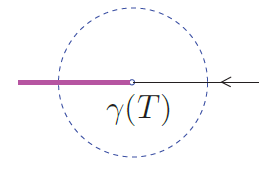
\includegraphics[width=0.3\textwidth]{./SaltChapter/fig-4-0-6}
\end{center}
%\caption{$\mathbb C$에 정의된 제곱급수의 수렴영역}
%\label{fig-4-0-3}
\end{figure*}

그런데 $\gamma(T)$는 $f$의 고립된 근이 아니므로
$\gamma(T)$를 중심으로 적당한 반지름 $\delta$의 원판에서
 $f(z)=0$이다. 즉, 
 $t$ 를 $T$에 가깝게 잡아 $|\gamma(t) - \gamma(T)|<r$을 만족하면
 $T$보다 큰 $t$에 대하여 $f(\gamma(t))=0$이 된다.
이는 $T$의 정의에 모순이다. 따라서 $T$는 $1$보다 작을 수 없어 증명이 끝난다.
\hfill $\square$

\begin{saltexample}[label=example-4-7]{}{}
$\cos z$와 $\sin z$의 정의로부터 모든 복소수 $z\in \mathbb C$에 대하여
$(\cos z)^2 + (\sin z)^2 = 1$임을 이미 알고 있다.
여기서는 정리의 결과를 이용하여 이를 증명해보자.
$f:\mathbb C \to \mathbb C$를 $f(z) = (\cos z)^2 + (\sin z)^2 - 1$로
정의하자. 그러면 $f$는 전해석함수이다. 또한
모든 $x\in \mathbb R$에 대하여 $ f(x) = (\cos x)^2 + (\sin x)^2 - 1 = 0$이다.
이제 정리를 적용하면 $\mathbb C$에서 $f\equiv 0$임을 알 수 있다.
\end{saltexample}

정리로부터 다음 결과를 바로 얻는다.

\begin{salt_corollary} [항등정리] \label{coro-4-6}
\
\begin{itemize}
\item[(1)] $D$가 영역이고,
\item[(2)] $f,g:D\to\mathbb C$가 $D$에서 복소해석함수이고,
\item[(3)] $D$의 서로 다른 점으로 만든 수열 $(z_n)_{n\in\mathbb N}$이 $z_*\in D$로 수렴하고,
$f(z_n) = g(z_n)$이면,
\end{itemize}
모든 $z\in D$에 대하여 $f(z) = g(z)$이다.
\end{salt_corollary}

{\bf 증명}

$z\in D$에 대하여
$h:D\to\mathbb C$를 $h(z) = f(z) - g(z)$로 정의하고
$z_n$을 복소해석함수 $h$의 근이라 하자.
정리의 결과로부터 $h$는 $D$에서 항등적으로 $0$이 되므로 증명이 끝난다.\hfill $\square$

\begin{saltexample}[label=example-4-8]{}{}
함수 $\exp:\mathbb C \to \mathbb C$
\[
\exp z = \exp(x+iy) := e^x (\cos y + i\sin y), \quad
z + x+iy\in \mathbb C
\]
는  전해석함수이고, $x\in \mathbb R$에서 $\exp x = e^x$를 만족한다.
다시 말하면, $\exp$ 함수는 실수에 정의된 지수함수를 복소수 전해석함수로 확장한 것이다.
전해석함수로 확장하는 다른 방법이 있을까? 그렇지 않다는 것을 보이자.
$g:\mathbb C \to \mathbb C$를  $x\in \mathbb R$에서 $g(x)=e^x$를 만족하는
전해석함수라고 가정하자.
그러면,
\[
\text{모든 } x\in \mathbb R \text{에 대하여 } \exp x = g(x).
\]
특히, 
\[
\exp\left(\dfrac1n\right)=  g\left(\dfrac1n\right), \quad n\in\mathbb N
\]
이고 $1/n \to 0\in \mathbb C$이다.
따라서 항등정리에 의해  모든 $z\in \mathbb C$에 대하여 $\exp z = g(z)$이다.
따라서 실수로 한정했을 때 $e^x$가 되는 전해석함수는 유일하다.
이 결과는 \ref{sec-1-4-1}의 복소 지수함수가 자연스러운 정의임을 설명해준다. 
\hfill $\diamondsuit$
\end{saltexample}

\begin{salt_exercise} \label{ex-4-22}
항등정리를 이용하여 모든 $z_1, z_2 \in \mathbb C$에 대하여
\[
\cos(z_1 + z_2) = (\cos z_1)(\cos z_2) - (\sin z_1)(\sin z_2)
\]
이 성립함을 보여라.
$z_1$, $z_2$가 실수인 경우에 성립함을 활용하라.
\end{salt_exercise}

\begin{salt_exercise} \label{ex-4-23}
영역  $D$에 정의된 복소해석함수의 집합을 $\Hol(D)$라 하자.
그러면 $z\in D$와 $f,g\in \Hol(D)$에 대한 점별 연산
\begin{align*}
(f+g)(z) &=f(z)+g(z), \\
(f\cdot g)(z) &=f(z)g(z)
\end{align*}
에 대하여 $\Hol(D)$가 가환환(commutative ring)이 됨을 쉽게 확인할 수 있다.
(가환환 $R$은 두 연산 $+$와 $\cdot$를 가지며
$(R,+)$는 가환군이고 $\cdot$는 교환법칙, 결합법칙을 만족하며
분배법칙도 성립한다. 즉, $a,b,c\in R$에 대하여 $(a+b)\cdot c = a\cdot c + b\cdot c$이다.)
$\Hol(D)$가 정역(integral domain)이 됨을 보여라.
즉, 영인자(zero divisor)를 갖지 않는다. 다시 말해 $f,g\in \Hol(D)$가 $f\cdot g=0$를
만족하면 $f=0$이거나 $g=0$이다.

$\Hol(D)$ 대신 $D$에 정의된 복소 연속함수의 집합 $C(D)$를 생각하면
$C(D)$도 점별 연산에 대하여 가환환이 된다.
$C(D)$도 정역인가?
(이 결과는 연속함수는 복소해석함수만큼 ``엄밀''하지 않음을 보여준다.)
\end{salt_exercise}

\begin{salt_exercise} \label{ex-4-24}
영역 $D$에서 $f,g$가 복소해석함수라 하자.
다음 중 어떤 조건이 영역 전체에서 $f=g$임을 보장하는가?
\begin{itemize}
\item[(1)] 
$D$의 서로 다른 점으로 된 수열 $(z_n)_{n\in\mathbb N}$이 존재하여
모든 $n\in \mathbb N$에서 $f(z_n) = g(z_n)$을 만족한다.
\item[(2)] $D$의 서로 다른 점으로 된 수열 $(z_n)_{n\in\mathbb N}$이 $D$의 한점으로 수렴하고
모든 $n\in \mathbb N$에서 $f(z_n) = g(z_n)$을 만족한다.
\item[(3)] $D$의 서로 다른 두 점 $a,b$를 연결하는 매끄러운 경로 $\gamma$에서
$f=g$이다.
\item[(4)]  $w\in D$이고, 모든 $n\ge0$에 대하여 $f^{(n)}(w) = g^{(n)}(w)$이다.
\end{itemize}
\end{salt_exercise}

\begin{salt_exercise} \label{ex-4-25}
$f$가 전해석함수라고 가정하자.
임의의 점 $z_0\in \mathbb C$에 대한 제곱급수 전개
$f(z) = \Sum_{n=0}^\infty c_n(z-z_0)^n$마다 적어도 하나의 계수가 $0$이다.
$f$는 다항식임을 증명하라.
\end{salt_exercise}

\section{최대절대값정리} \label{sec-4-6}

이 절에서는 복소해석학의 중요한 결과인  최대절대값정리를 증명할 것이다.
이는 상수함수가 아닌 복소해석함수 $f:D\to\mathbb C$의 절대값 $|f|$는 영역 $D$에서
최대값을 가질 수 없음을 의미한다.

\begin{salttheorem} [최대절대값정리] {}{} \label{thm-4-6}

\begin{itemize}
\item[(1)] $D$가 영역이고,
\item[(2)] $f:D\to\mathbb C$가 $D$에서 복소해석함수이고,
\item[(3)] 모든 $z\in D$에 대하여 $|f(z_0)| \ge |f(z)|$를 만족하는 $z_0\in D$가 존재하면,
\end{itemize}
$f$는 $D$에서 상수함수이다.
\end{salttheorem}

{\bf 증명}

중심이 $z_0$이고 반지름 $2r$인 원판이 영역 $D$에 포함되는 $r>0$을 잡고,
$C_r$을 $C_r(t) = z_0 + r\exp(it)$ ($t\in [0,2\pi]$)로 정의된 원형 경로라 하자.
그러면, 코시 적분공식에 의해,
\begin{align*}
f(z_0) &= \dfrac1{2\pi i} \int_\gamma \dfrac{f(z)}{z-z_0}dz
=  \dfrac1{2\pi i} \int_0^{2\pi} \dfrac{f(z_0 + r\exp(it))}{r\exp(it)} ir\exp(it)dt \\
&=  \dfrac1{2\pi} \int_0^{2\pi} f(z_0 + r\exp(it))dt
\end{align*}
이며, 여기서 마지막 식은 $C_r$에서 $f$의 ``평균''으로 해석할 수 있다.
모든 $t$에 대하여 $|f(z_0 + r\exp(it))| \le |f(z_0)|$이므로
\begin{align*}
|f(z_0)| = \left|\dfrac1{2\pi} \int_0^{2\pi} f(z_0 + r\exp(it))dt \right| 
&\le \dfrac1{2\pi} \int_0^{2\pi}  \left| f(z_0 + r\exp(it)) \right|  dt \\
& \le \dfrac1{2\pi} \int_0^{2\pi}  \left| f(z_0) \right|  dt  = |f(z_0)|.
\end{align*}
이 식에서 부등호 $\le$는 모두 등호로 바뀔 수 있거 정리하면
\[
 \dfrac1{2\pi} \int_0^{2\pi}  \big( 
 \underbrace{|f(z_0)|  - |f(z_0 + r\exp(it))|}_{\ge0} \big)  dt  = 0.
\]
를 얻는다.
피적분함수가 $0$보다 크거나 같기 때문에 
모든 $t$에 대하여 $|f(z_0 + r\exp(it))|=|f(z_0)|$이다.
$r$을 더 작은 값으로 바꾸어도 같은 결과를 얻는다.
따라서 $f$는 
원판 $\Delta:= \{z \in \mathbb C \,:\, |z-z_0| \le r \}$을
원 $\{ w\in \mathbb C\,:\, |w| = |f(z_0)| \}$위로 보낸다.
연습문제 \ref{ex-2-11}의 결과로부터
$f$는 $\Delta$에서 상수함수이다.
따라서 항등정리를 적용하면 $f$는 $D$ 전체에서  상수함수이다.
\hfill $\square$

\begin{saltexample}[label=example-4-9]{}{}
$\mathbb H := \{z\in\mathbb C\,:\, \Re(z)\ge 0\}$를 우측 반평면이라 하고
$f:\mathbb H\to \mathbb C$를 다음과 같이 정의하자.
\[
f(z) =  \dfrac{\exp(-z)}{z+1}, \quad z\in\mathbb H.
\]
그러면 다음 최대값이 존재한다.
\[
\|f\|_\infty := \max_{z\in\mathbb H} |f(z)|.
\]
최대값의 존재성에 대한 우려를 잊고,
일단 존재한다는 가정하에, 최대절대값정리가 어떻게 그 값을 계산하는데 도움을 주는지  살펴보자.
$z_0\in \mathbb H$에서 최대값을 갖는다고 가정하자.
그러면 최대절대값정리로부터 $z_0$의 실수부는 양수가 될 수 없다.
따라서 $z_0 \in i\mathbb R$이고, 어떤 $y_0\in\mathbb R$에 대하여 $z_0=iy_0$라 하자.
한편,
\[
|f(iy)| = \left| \dfrac{\exp(-iy)}{iy+1} \right| = \dfrac1{\sqrt{y^2+1}}, y\in\mathbb R.
\]
따라서
$\|f\|_\infty = \max\limits_{z\in\mathbb H} |f(z)|
= \max\limits_{y\in\mathbb R} |f(iy)| 
= \max\limits_{y\in\mathbb R} \dfrac1{\sqrt{y^2+1}} 
= \dfrac1{\sqrt{0^2+1}} = 1$. \hfill $\diamondsuit$
\end{saltexample}

\begin{salt_exercise} \label{ex-4-26}
영역 $D$에서 $f:D\to \mathbb C$가 상수함수가 아닌 복소해석함수라 하자.
그러면 $z\mapsto |f(z)|$를 최대로 하는 점이 $D$에 존재하지 않음을 보여라.
\end{salt_exercise}

\begin{salt_exercise} [최소절대값정리] \label{ex-4-27}
영역 $D$에서 $f:D\to \mathbb C$가 복소해석함수라 하자.
모든 $z\in D$에 대하여 $|f(z_0)| \le |f(z)|$를 만족하는 $z_0\in D$가 존재한다고 하자.
그러면 $f(z_0)=0$이거나 $f$는 $D$에서 상수함수임을 증명하라.
\end{salt_exercise}

\begin{salt_exercise} \label{ex-4-28}
함수 $f(z)=z^2-2$에 대하여
$\{z\in\mathbb C \,:\, |z|\le 1\}$에서 $|f(z)|$의 최댓값과 최솟값을 구하라.
\end{salt_exercise}

\section{로랑 급수}

로랑(Laurent) 급수는 테일러 급수의 일반화이다. 
테일러 급수
\[
\sum_{n=0}^\infty c_n(z-z_0)^n
\]
는 $z-z_0$의 음의 지수를 갖지 않으며 적당한 원판에서 수렴하는데,
로랑 급수는
\[
\sum_{n\in \mathbb Z} c_n(z-z_0)^n
= \cdots + c_{-1}(z-z_0)^{-1} + c+0 + c_1(z-z_0)^1 + \cdots
\]
는 $z-z_0$의 음의 지수도 갖는다.

\begin{figure*}[h!]
\begin{center}
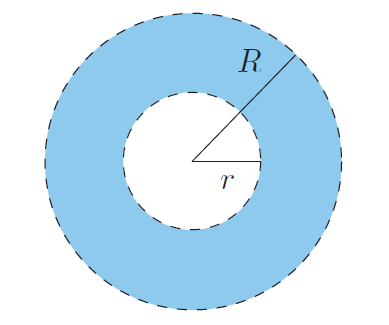
\includegraphics[width=0.3\textwidth]{./SaltChapter/fig-4-0-7}
\end{center}
%\caption{$\mathbb C$에 정의된 제곱급수의 수렴영역}
%\label{fig-4-0-3}
\end{figure*}

앞으로 다음을 살펴볼 예정이다.
\begin{itemize}
\item[(1)] 로랑 급수는 $z_0$ 중심의 
원환 $\{ z\in \mathbb C \,:\, r < |z-z_0| <R\}$에서 ``수렴''하는
복소해석함수가 된다.
\item[(2)] 역으로, $z_0$를 중심으로 하는 원환에 정의된 복소해석함수가
특이점을 원환의 안쪽 구멍에서만 갖는다면
함수는 원환에서 로랑급수를 갖는다. 예를 들어 모든 $z\in \mathbb C$에 대하여
\[
\exp z = 1 + \dfrac{z}{1!} + \dfrac{z^2}{2!} + \dfrac{z^3}{3!} + \cdots
\]
이고 $z\ne0$에 대한 ``로랑 급수 전개''는
\[
\exp \dfrac1z = 1 + \dfrac{1}{z} + \dfrac{1}{2!}\dfrac1{z^2} + \dfrac{1}{3!}\dfrac1{z^3} + \cdots.
\]
$\exp(1/z)$는 $\mathbb C\setminus \{0\}$에서 복소해석함수이다.
$\mathbb C\setminus \{0\}$는 원환의 퇴화된 모습으로
중심이 $0$이고 안쪽 반지름 $r=0$, 바깥쪽 반지름 $R=+\infty$인 경우다.
\end{itemize}

우선 $\Sum_{n\in \mathbb Z} c_n(z-z_0)^n$의 수렴에 대한 개념부터 만들자.

\begin{saltdefinition}{}{} \label{def-4-3}
\[
\Sum_{n=1}^\infty c_{-n}(z-z_0)^n, \quad
\Sum_{n=0}^\infty c_{n}(z-z_0)^n
\]
이 모두 수렴하면, 
로랑 급수  $\Sum_{n\in \mathbb Z} c_n(z-z_0)^n$가 수렴한다.

$\Sum_{n\in \mathbb Z} c_n(z-z_0)^n$가 수렴하면, 다음과 같이 쓸 수 있고
\[
\Sum_{n\in \mathbb Z} c_n(z-z_0)^n
= \Sum_{n=1}^\infty c_{-n}(z-z_0)^n + \Sum_{n=0}^\infty c_{n}(z-z_0)^n
\]
는 로랑 급수의 합이라 부른다.
\end{saltdefinition}

\begin{saltexample}[label=example-4-10]{}{}
어떤 $z\in \mathbb C$에 대하여 로랑 급수
\[
\cdots + \dfrac1{8z^3} + \dfrac1{4z^2} + \dfrac1{2z} + 1 + z^2 + z^3 + \cdots
\]
가 수렴할까? 
\begin{itemize}
\item[(1)] $1 + z^2 + z^3 + \cdots$은 $|z|<1$에서 수렴하고, $|z|>1$에서 발산한다.
\item[(2)] $\dfrac1{2z} + \dfrac1{4z^2} +  \dfrac1{8z^3} + \cdots$는
$\left|\dfrac1{2z}\right|<1$에서 수렴하고, $\left|\dfrac1{2z}\right|>1$에서 발산한다.
\end{itemize}
즉, 이 로랑 급수는 $|z|<1$과 $|z|>1/2$를 모두 만족하는 경우 수렴하므로
원환 $\{ z\in \mathbb C\,:\, 1/2<|z|<1\}$에서 수렴하고,
$|z|>1$이거나 $|z|<1/2$이면 발산한다.
\hfill  $\diamondsuit$
\end{saltexample}

{\bf 어떤 $z$에 대하여 $\Sum_{n\in \mathbb Z} c_n(z-z_0)^n$이 수렴할까?}

\begin{itemize}
\item[(1)] 정리 \ref{thm-4-1}에 의하면
$\Sum_{n=0}^\infty c_n(z-z_0)^n$가
$|z-z_0|<R$에서 수렴하고,  $|z-z_0|>R$에서 발산하는  상수 $R$이 존재한다.
\item[(2)] $\Sum_{n=1}^\infty c_{-n}(z-z_0)^{-n}$은 어떨까?
제곱급수 $\Sum_{n=1}^\infty c_{-n}w^n$도 $|w|<\tilde R$에서 수렴하고
$|w|>\tilde R$에서 발산한다. 따라서,
$w:= (z-z_0)^{-1}$로 두면, $\Sum_{n=1}^\infty c_{-n}(z-z_0)^{-n}$은 
$1/|z-z_0| <\tilde R$에서 수렴한다. 즉, $|z-z_0|>1/\tilde R=:r$에서 수렴,
$|z-z_0|<r$에서 발산한다.
\end{itemize}

따라서 로랑 급수는 원환  $\{ z\in \mathbb C \,:\, r < |z-z_0| <R\}$에서 수렴하고
$|z-z_0|<r$이거나 $|z-z_0|>R$일 때 발산한다.

{\bf  수렴하는 원판에서 제곱급수는 복소해석함수일까?}

\begin{itemize}
\item[(1)] $z\mapsto \Sum_{n=0}^\infty c_{n}(z-z_0)^n$은
$\{ z\in\mathbb C\,:\, |z-z_0| <R\}$에서 복소해석함수이다. 따라서,
 원환  $\{ z\in \mathbb C \,:\, r < |z-z_0| <R\}$에서도 복소해석함수이다.
\item[(2)] 함수
\[
w \stackrel{g}{\mapsto} \Sum_{n=1}^\infty c_{-n}w^n
\]
는 $\{ w\in\mathbb C\,:\, |w| < \tilde R \}$에서 복소해석함수이다.
또한, 함수 $z \stackrel{f}{\mapsto} (z-z_0)^{-1}: \mathbb C \setminus \{z_0\} \to \mathbb C$도
복소해석함수이다.
그러므로 합성함수 $g\circ f$는 $\{ z\in\mathbb C\,:\, |z-z_0| >r \}$에서
복소해석함수이다. 즉,
\[
z \stackrel{g\circ f}{\mapsto} \Sum_{n=1}^\infty c_{-n}(z-z_0)^{-n}
\]
이 $\{ z\in\mathbb C \,:\, r<|z-z_0| \}$에서 복소해석함수이다. 
특히 원환  $\{ z\in \mathbb C \,:\, r < |z-z_0| <R\}$에서도 복소해석함수이다.
\end{itemize}

따라서 합으로 정의된 함수
$z \mapsto \Sum_{n=0}^\infty c_n(z-z_0)^n + \Sum_{n=1}^\infty c_{-n}(z-z_0)^{-n}
= \Sum_{n\in \mathbb Z} c_n(z-z_0)^n$는 
원환
$\{ z\in \mathbb C \,:\, r < |z-z_0| <R\}$에서 복소해석함수이다.

요약하면,
로랑 급수 
$\Sum_{n\in \mathbb Z} c_n(z-z_0)^n$는 
적당한 $r, R$에 대하여
원환\footnote{공집합이 될 수도 있다!}
$\{ z\in \mathbb C \,:\, r < |z-z_0| <R\}$에서 복소해석함수이고
함수 
\[
z \mapsto \Sum_{n\in \mathbb Z} c_n(z-z_0)^n
\]
는 원환$\{ z\in \mathbb C \,:\, r < |z-z_0| <R\}$에서 
복소해석함수임을 살펴보았다.

역으로 원환에서 정의된 복소해석함수는 로랑 급수 전개를 가짐을 다음 정리로부터 알 수 있다.

\begin{salttheorem}{}{} \label{thm-4-7}
$f$가 $\mathbb A:= \{ z\in \mathbb C \,:\, r < |z-z_0| <R\}$에서 복소해석함수이면,
\begin{equation}\label{eq-4-5}
f(z) = \Sum_{n\in \mathbb Z} c_n(z-z_0)^n, \quad z\in\mathbb A
\end{equation}
이다. 여기서
\begin{itemize}
\item[(1)] $c_n = \dfrac1{2\pi i} \dint_C \dfrac{f(\zeta)}{(\zeta - z_0)^{n+1}} d\zeta$,
\item[(2)] $C$는 $C(t) = z_0 + \rho \exp(it)$ ($t\in [0,2\pi]$)로 정의된 원형 경로,
\item[(3)] $\rho$는 $r<\rho<R$인 임의의 실수이다.
\end{itemize}
또한, 식 \eqref{eq-4-5}의 계수는 유일하게 결정된다.
\end{salttheorem}

\begin{saltexample}[label=example-4-11]{}{}
함수 $f:\mathbb C\setminus \{0\} \to \mathbb C$를
$f(z) = z^3\exp(1/z)$ ($z\ne0$)로 정의하자.
그러면, $f$는 $\mathbb A:= \{ z\in \mathbb C \,:\,  0 <|z| <+\infty \}$에서
복소해석함수이다. 따라서 정리의 결과를 적용하면
$f$는 로랑 급수
\[
\sum_{n\in\mathbb Z} c_n z^n
\]
을 갖는다. 
계수를 직접 찾아보면
\[
\exp \dfrac 1z = 1 + \dfrac1z + \dfrac1{2!z^2} + \cdots, \quad z\ne0
\]
이므로
$f(z) = z^3 \exp \dfrac 1z = z^3 + z^2 + \dfrac 1{2!} + \dfrac1{3!}
+ \dfrac1{4!z} + \cdots$ ($z\ne 0$)를 얻는다.
따라서,
\[
\ldots, c_{-1} = \dfrac1{4!}, c_0 = \dfrac1{3!}, c_1 = \dfrac1{2!}, c_2 = 1, c_3 = 1,
\]
이고 $n\ge4$에 대하여 $c_n=0$이다.
\hfill $\diamondsuit$
\end{saltexample}

{\bf 증명 (정리 \ref{thm-4-7})} (존재성).

$z\in \mathbb A$를 고정하자.
$r < \tilde r < |z-z_0| <\tilde R <R$을 만족하는 $\tilde r$과  $\tilde R$을 선택한다.
$t\in [\theta, 2\pi + \theta]$, $\theta:= Arg(z) + \pi/2$에 대하여
원형 경로 $\gamma_1$과  $\gamma_2$를 
\begin{align*}
\gamma_1(t) &= z_0 + \tilde r \exp (it),\\
\gamma_2(t) &= z_0 + \tilde R \exp (it)
\end{align*}
라고 하자. 
$\gamma_3: [\tilde r, \tilde R] \to \mathbb A$는 경로
\[
\gamma_3(t) = ti\dfrac{z-z_0}{|z-z_0|}
\]
라 하자. (이 경로는 $\gamma_1$과 $\gamma_2$를 잇는 직선 경로이다.
$i$를 곱한 것은 $z$를 피하기 위해 $90^\circ$ 회전을 의미한다.)
그림 \ref{fig-4-2}를 참고하라.

\begin{figure}[h!]
\begin{center}
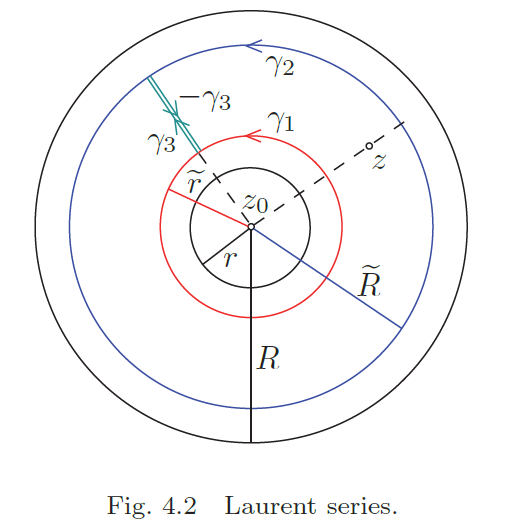
\includegraphics[width=0.4\textwidth]{./SaltChapter/fig-4-2}
\end{center}
\caption{로랑 급수}
\label{fig-4-2}
\end{figure}

당연히
경로 $\gamma := \gamma_2 - \gamma_3 - \gamma_1 + \gamma_3$는
$z$를 중심으로 하는 작은 원 $C_\delta$와 $\mathbb A\setminus \{z\}$-호모토픽하다.
또한, $\dfrac{f(\cdot)}{\cdot-z}$는 $\mathbb A\setminus \{z\}$에서
복소해석함수이므로
\[
\int_\gamma \dfrac{f(\zeta)}{\zeta-z} d\zeta
= \int_{C_\delta} \dfrac{f(\zeta)}{\zeta-z} d\zeta
= f(z) \cdot 2\pi i,
\]
여기서 첫번째 등호는 코시 적분정리로부터,
두번째 등호는 코시 적분공식로부터 얻어진다.
$\gamma_3$를 따른 경로적분은 $-\gamma_3$에서의 경로적분과 상쇄된다.
\begin{align*}
f(z) &= \dfrac1{2\pi i} \int_\gamma \dfrac{f(\zeta)}{\zeta-z}d\zeta
= \dfrac1{2\pi i} \int_{\gamma_2} - \cancel{ \int_{\gamma_3}}
-  \int_{\gamma_1} + \cancel{\int_{\gamma_3 }}\dfrac{f(\zeta)}{\zeta-z}d\zeta \\
&= \underbrace{\dfrac1{2\pi i} \int_{\gamma_2} \dfrac{f(\zeta)}{\zeta-z}d\zeta}_{\text{(I)}}
- \underbrace{\dfrac1{2\pi i} \int_{\gamma_1} \dfrac{f(\zeta)}{\zeta-z}d\zeta}_{(\text{(II)}}.
\end{align*}
이제 적분 (I)은
\[
\sum_{n=0}^\infty c_n(z-z_0)^n
\]
으로 적분 (II)는 
\[
\sum_{n=1}^\infty c_{-n}(z-z_0)^{-n}
\]
으로 표현되고 이를 합하면 $f$의 로랑 급수 전개를 얻는다는 것을 보이자.

{\bf 단계 1}.
이 단계에서는 $\dfrac1{2\pi i} \dint_{\gamma_2} \dfrac{f(\zeta)}{\zeta-z}d\zeta
= \Sum_{n=0}^\infty c_n(z-z_0)^n$을 증명하자.

$\zeta \in \gamma_2$에 대하여
\[
\dfrac{f(\zeta)}{\zeta-z} = \dfrac{f(\zeta)}{\zeta-z_0+z_0-z}
= \dfrac{f(\zeta)}{(\zeta-z_0)\left(1 - \dfrac{z-z_0}{\zeta- z_0}\right)}
= \dfrac{f(\zeta)}{(\zeta-z_0)(1-w)},
\]
여기서 $w:= \dfrac{z-z_0}{\zeta- z_0}$이다.
$|w| = \dfrac{|z-z_0|}{|\zeta- z_0|} = \dfrac{|z-z_0|}{\tilde R} < 1$이므로
\[
\dfrac1{1-w} = 1+ w + w^2 + w^3 + \cdots + w^{n-1} + \dfrac{w^n}{1-w}.
\]
피적분함수를 다시 쓰면,
\begin{align*}
\dfrac{f(\zeta)}{\zeta-z} &= \dfrac{f(\zeta)}{\zeta-z_0} \left(
1+ w + \cdots + w^{n-1} + \dfrac{w^n}{1-w} \right) \\
&= \dfrac{f(\zeta)}{\zeta-z_0} + \cdots \dfrac{f(\zeta)}{(\zeta-z_0)^n}(z-z_0)^{n-1}
+ \dfrac{f(\zeta)(z-z_0)^n}{(\zeta-z_0)^n(\zeta-z)}.
\end{align*}
따라서 적분은
\begin{align*}
\dfrac1{2\pi i} \int_{\gamma_2} \dfrac{f(\zeta)}{\zeta-z} d\zeta
&= \dfrac1{2\pi i} \int_{\gamma_2} \dfrac{f(\zeta)}{\zeta-z_0} d\zeta
+ \cdots + \dfrac1{2\pi i} \int_{\gamma_2} \dfrac{f(\zeta)}{(\zeta-z_0)^n} d\zeta 
\cdot (z-z_0)^{n-1} \\
& \quad\quad + \dfrac1{2\pi i} \int_{\gamma_2} \dfrac{f(\zeta)}{(\zeta-z_0)^n(\zeta-z)} d\zeta
\cdot (z-z_0)^{n}  \\
&= c_0 + c_1(z-z_0) + \cdots + c_{n-1}(z-z_0)^{n-1} + R_n(z),
\end{align*}
여기서, 
\[
R_n(z) := \dfrac1{2\pi i} \int_{\gamma_2} \dfrac{f(\zeta)(z-z_0)^n}{(\zeta-z_0)^n(\zeta-z)} d\zeta.
\]
이 계산과정에서 $\gamma_2$가 중심이 $z_0$이고 반지름 $\rho$ ($r<\rho<R$)인
임의의 원과 $\mathbb A$-호모토픽함을 이용했다.
정리 \ref{thm-3-4}에 의해
\[
\dfrac1{2\pi i} \int_{\gamma_2} \dfrac{f(\zeta)}{(\zeta-z_0)^k} d\zeta
= \dfrac1{2\pi i} \int_{C} \dfrac{f(\zeta)}{(\zeta-z_0)^k} d\zeta
= c_{k-1},
\quad k=1,\ldots, n.
\]
이제 
$\Lim_{n\to\infty} R_n = 0$만 보이면,
원하는 식을 얻는다.
\[
\dfrac1{2\pi i} \dint_{\gamma_2} \dfrac{f(\zeta)}{\zeta-z}d\zeta
= \Sum_{n=0}^\infty c_n(z-z_0)^n.
\]
모든 $\zeta \in \gamma_2$에 대하여 $|f(\zeta)| <M$인 $M>0$이 존재한다.
또한 $|\zeta - z_0| = \tilde R$이고,
\[
|\zeta - z| = |\zeta - z_0 - (z-z_0) | \ge
|\zeta - z_0| - |z-z_0| = \tilde R - |z-z_0|
\]
이므로 
\[
|R_n(z)| \le \left( \dfrac{|z-z_0|}{\tilde R} \right)^n
\dfrac{M\tilde R}{\tilde R - |z-z_0|} 
\stackrel{n\to\infty}{\longrightarrow} 0.
\]
결론적으로 
$c_0 + c_1(z-z_0) + c_2(z-z_0)^2 + c_3(z-z_0)^3 + \cdots
= \dfrac1{2\pi i } \dint_{\gamma_2} \dfrac{f(\zeta)}{\zeta-z}d\zeta$.


{\bf 단계 2}. 이 단계에서는
$ - \dfrac1{2\pi i } \dint_{\gamma_1} \dfrac{f(\zeta)}{\zeta-z}d\zeta
\sum_{n=1}^\infty c_{-n}(z-z_0)^{-n}$를 보이자.
\begin{align*}
-\dfrac1{2\pi i } \dint_{\gamma_1} \dfrac{f(\zeta)}{\zeta-z}d\zeta
&= \dfrac1{2\pi i } \dint_{\gamma_1} \dfrac{f(\zeta)}{(\zeta-z_0) - (\zeta-z_0)}d\zeta \\
&= \dfrac1{2\pi i } \dint_{\gamma_1} \dfrac{f(\zeta)}{(z-z_0)
\left(1 - \dfrac{\zeta-z_0}{z-z_0}\right)}d\zeta
\end{align*}
에서 $w:= \dfrac{\zeta-z_0}{z-z_0}$라 두면,
$|w| = \dfrac{\tilde r}{|z-z_0|} <1$이므로
\[
\dfrac1{1 - \dfrac{\zeta-z_0}{z-z_0}}
= \dfrac1{1-w} = 1+ w + w^2 + w^3 + \cdots + w^{n-1} + \dfrac{w^n}{1-w}.
\]
따라서
\begin{align*}
-\dfrac1{2\pi i } & \dint_{\gamma_1} \dfrac{f(\zeta)}{\zeta-z}d\zeta \\
& = \dfrac1{2\pi i } \dint_{\gamma_1} f(\zeta) \left(
\dfrac1{z-\zeta} + \cdots + \dfrac{(\zeta-z_0)^{n-1}}{(z-z_0)^n}
+ \dfrac{(\zeta - z_0)^n}{(z-z_0)^n(z-\zeta)} \right) d\zeta \\
&=\dfrac1{2\pi i }  \dint_{\gamma_1} f(\zeta)d\zeta \cdot \dfrac1{z-z_0} 
+ \cdots + \dfrac1{2\pi i } \dint_{\gamma_1} \dfrac{f(\zeta)}{(\zeta-z_0)^{-n+1}} d\zeta
\cdot\dfrac1{(z-z_0)^n} \\
&\quad \quad + \dfrac1{2\pi i } \dint_{\gamma_1} 
\dfrac{f(\zeta)(\zeta-z_0)^n}{(\zeta-z_0)^n(z-\zeta)} d\zeta \\
& = c_{-1}(z-z_0)^{-1} + \cdots + c_{-n}(z-z_0)^{-n} + \tilde R_n(z),
\end{align*}
여기서, 
\[
\tilde R_n(z) := \dfrac1{2\pi i} \int_{\gamma_1} \dfrac{f(\zeta)(\zeta-z_0)^n}{(z-z_0)^n(z-\zeta)} d\zeta.
\]
이 계산과정에서 $\gamma_1$이 중심이 $z_0$이고 반지름 $\rho$ ($r<\rho<R$)인
임의의 원과 $\mathbb A$-호모토픽함을 이용했다.
정리 \ref{thm-3-4}에 의해
\[
\dfrac1{2\pi i} \int_{\gamma_1} \dfrac{f(\zeta)}{(\zeta-z_0)^k} d\zeta
= \dfrac1{2\pi i} \int_{C} \dfrac{f(\zeta)}{(\zeta-z_0)^k} d\zeta
= c_{k-1},
\quad k=0,-1,\ldots, -n+1.
\]
이제 
$\Lim_{n\to\infty} \tilde R_n = 0$만 보이면,
원하는 식을 얻는다.
모든 $\zeta \in \gamma_1$에 대하여 $|f(\zeta)| <M$인 $M>0$이 존재한다.
또한 $|\zeta - z_0| = \tilde r$이고,
\[
|z-\zeta| = |(z-z_0) -(\zeta - z_0) | \ge
|z- z_0| - |\zeta-z_0| =  |z-z_0| - \tilde r
\]
이므로 
\[
|\tilde R_n(z)| \le \left( \dfrac{\tilde r}{|z-z_0|} \right)^n
\dfrac{M \tilde r}{|z-z_0| - \tilde r} 
\stackrel{n\to\infty}{\longrightarrow} 0.
\]
결론적으로 
$c_{-1}(z-z_0)^{-1} +\cdots + c_{1(n-1)} (z-z_0)^{-(n-1)} + \cdots
= - \dfrac1{2\pi i } \dint_{\gamma_1} \dfrac{f(\zeta)}{\zeta-z}d\zeta$.
이로써 로랑 급수 전개의 존재성을 증명하였다.

{\bf 계수들의 유일성}.
코시 적분공식을 이용하여 로랑 급수가 유일함을 보이자. 즉,
\[
f(z) = \sum_{n\in\mathbb Z} \tilde c_n(z-z_0)^n, \quad
r < |z-z_0| <R
\]
이면, 모든 $n$에 대하여 $\tilde c_n = c_n$이다.
$n\ne 1$이면, $(z-z_0)^n = \dfrac d{dz} \left( \dfrac{(z-z_0)^{n+1}}{n+1} \right)$이므로
\[
\int_C (z-z_0)^n dz = 0 \quad (n\ne1),
\]
여기서 $C$는 $C(t)=z_0 + \rho\exp(it)$ ($t\in[0,2\pi]$)로 주어진 경로이다.
직접 계산하는 방법으로
\[
\int_C \dfrac1{z-z_0} dz = \int_0^{2\pi} \dfrac1{r\exp(it)}ir\exp(it)dt = 2\pi i.
\]
따라서 원환에서 항별 적분을 적용할 수 있다면,
\[
\int_C (z-z_0)^{-m-1} \sum_{n\in\mathbb Z} \tilde c (z-z_0)^n dz
= \sum_{n\in\mathbb Z} \tilde c \int_C (z-z_0)^{n-m-1} dz = 2\pi i \tilde c_m
\]
이 되므로 계수의 유일성을 얻는다.
이제 항별 적분이 가능함을 보아자.
\begin{align*}
 \sum_{n\in\mathbb Z} \tilde c (z-z_0)^{n-m-1}
 &= \left( \cdots + \dfrac{\tilde c_{m-2}}{(z-z_0)^3} +  \dfrac{\tilde c_{m-1}}{(z-z_0)^2} \right) \\
 & \quad + \dfrac{\tilde c_m}{z-z_0} + (\tilde c_{m+1} + \tilde c_{m+2}(z-z_0) + \cdots) \\
 & = f_1(z) + \dfrac{\tilde c_m}{z-z_0} + f_2(z).
\end{align*}
$f_1$과 $f_2$가 원환에서 부정적분을 가짐을 보이면 된다. 그러면, 원하는 결과로
\begin{align*}
\int_C  \sum_{n\in\mathbb Z} \tilde c (z-z_0)^{n-m-1} dz
&= \int_C \left( f_1(z) + \dfrac{\tilde c_m}{z-z_0} + f_2(z) \right) dz \\
&= 0 + 2\pi i \tilde c_m + 0 = 2\pi i \tilde c_m.
\end{align*}
을 얻는다.
$|z-z_0|<R$에서 $f_2(z) = \Sum_{n=1}^\infty \tilde c_{m+n} (z-z_0)^{n-1}$이고
\[
F_2(z) := \Sum_{n=1}^\infty \dfrac{\tilde c_{m+1}}n (z-z_0)^n,
\quad |z-z_0|<R
\]
이면, $\dfrac d{dz} F_2(z) = f_2(z)$가 되어 $F_2$는 $f_2$의 부정적분이 된다.
$f_1$에 대하여 
\[
f_1(z) = \sum_{n=1}^\infty \dfrac{\tilde c_{m-n}}{(z-z_0)^{n+1}} 
= \sum_{n=1}^\infty \tilde c_{m-n} w^{n+1},
\]
$w = \dfrac1{z-z_0}$이다. $R>|z-z_0| >r$에서 유효하므로
\[
\sum_{n=1}^\infty \tilde c_{m-n} w^{n+1}
\]
은 $|w|<\dfrac1r$에서 수렴한다. 
\[
G(w) = - \sum_{n=1}^\infty \dfrac{\tilde c_{m-n}}n w^n,\quad
|w|<\dfrac1r
\]
이라 하면, $\dfrac d{dz} G(w) = - \Sum_{n=1}^\infty \tilde c_{m-n} w^{n-1}$이다. 
이제 모든 $z\in \mathbb A$에 대하여
\[
F_1(z) = G\left(\dfrac1{z-z_0}\right) 
= - \Sum_{n=1}^\infty\dfrac{\tilde c_{m-n}}n (z-z_0)^{-n}
\]
로 정의하면,
\begin{align*}
\dfrac d{dz} F_1(z)
&= \left( G'\left(\dfrac1{z-z_0}\right)\right) \left(- \dfrac1{(z-z_0)^2}\right) \\
&= (z-z_0)^{-2} \sum_{n=1}^\infty \tilde c_{m-n} (z-z_0)^{-n+1} = f_1(z).
\end{align*}
\hfill $\square$

계수의 유일성은 고정된 원환에 대해서만 유효하다.
같은 함수라도 다른 원환들에서 유효하도록 로랑 급수를 전개하면
다른 로랑 급수를 얻는다.

\begin{saltexample}[label=example-4-12]{}{}

함수 $f$를 $\mathbb C\setminus\{0,1\}$에서
$f(z) = \dfrac1{z(z-1)}$로 정의하자. 

%\begin{figure}[h!]
\begin{center}
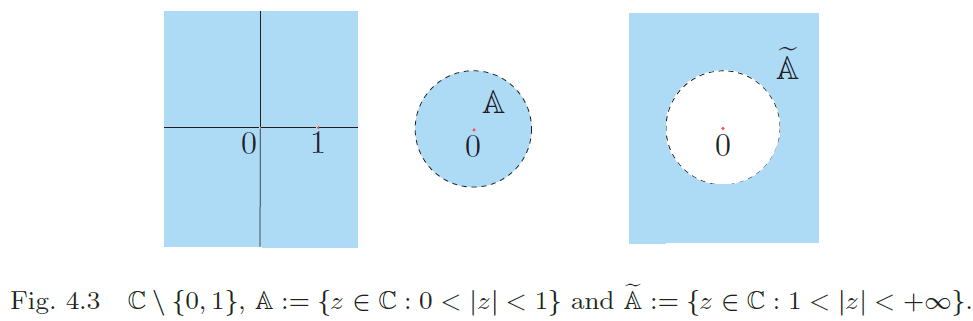
\includegraphics[width=0.7\textwidth]{./SaltChapter/fig-4-3}
\end{center}
\captionof{figure}{영역 $\mathbb C\setminus \{0,1\}$,
$\mathbb A:=\{ z\in \mathbb C\,:\, 0<|z|<1 \}$,
$\tilde {\mathbb A}:=\{ z\in \mathbb C\,:\, 1<|z|<\infty \}$.}
\label{fig-4-3}
%\end{figure}
$f$는 원환 $\mathbb A:=\{ z\in \mathbb C\,:\, 0<|z|<1 \}$에서
복소해석함수이다. 그 로랑 급수를 구하면?
$|z|<1$이므로
\[
f(z) = \dfrac1{z(z-1)} %= \dfrac1{z^2(1-1/z)}
= - \dfrac1z \left(1+z+z^2+ z^3 + \cdots \right)
= -\dfrac1z -1 -z -z^2 -z^3 - \cdots
\]
로 쓸 수 있기 때문에
계수를 구하면
\begin{align*}
c_{-2} &= c_{-3} = \cdots = 0, \\
c_{-1} & = c_0 = c_1 = \cdots = -1.
\end{align*}
그런데 $f$는 안쪽 반지름이 $1$이고 바깥쪽 반지름이 무한대인
원환 $\tilde{\mathbb A}:=\{ z\in \mathbb C\,:\, 1<|z| \}$에서도
복소해석함수이다. 따라서
$f$는 $\tilde{\mathbb A}$에서도 로랑 급수 전개가 가능하다.
$|z|>1$에서
\begin{align*}
f(z) = \dfrac1{z(z-1)} = \dfrac1{z^2(1-1/z)}
&= \dfrac1{z^2} \left( 1+ \dfrac1z + \dfrac1{z^2} + \dfrac1{z^3} + \cdots \right) \\
&= \dfrac 1{z^2} + \dfrac1{z^3} + \cdots
\end{align*}
이므로 로랑 급수의 계수는 다음과 같다.
\begin{align*}
\tilde c_{-2} &= \tilde c_{-3} = \cdots = 1, \\
\tilde c_{-1} & = \tilde c_0 = \tilde c_1 = \cdots = 0.
\end{align*}
두 가지 로랑 급수의 계수가 다르게 나오는데 놀라운 일이 아니다.
왜냐하면 다른 원환에서 로랑 급수를 전개했기 때문이다.
\hfill $\diamondsuit$
\end{saltexample}

\begin{salt_exercise}\label{ex-4-29}
예제 \ref{example-4-12}를 다시 생각해보자.
원환 ${\mathbb A_1}:=\{ z\in\mathbb C\,:\, 0 <|z-1|<1\}$과
원환 $\tilde{\mathbb A_1}:=\{ z\in\mathbb C\,:\, 1<|z-1|\}$에서
$f$의 로랑 급수를 구하라.
\end{salt_exercise}

\section{특이점의 분류}\label{sec-4-8}

다음 세 함수
\[
\dfrac{\sin z}{z}, \quad \dfrac1{z^3}, \quad \exp \dfrac1z
\]
는 모두 $0$에서 정의되지 않기 때문에
$0$을 이 함수들의 ``특이점(singularity)''이라 부른다.
그런데 특이점 근방에서 세 함수의 특성은 매우 다르다.
즉, {|bf 특이점의 본질}은 각 경우에서 모두 다르다.
우리는 각각의 경우 함수가 특이점 근방에서 어떻게 되는지를 
상세하게 살펴볼 예정인데 이를 특이점의 분류라 한다.
또한, 특이점의 종류를 쉽게 판별하는 분류법 2가지를 보게 될 것인데,
하나는 극한을 이용하여 특이점을 규명하는 방법이고
다른 하나는 로랑 급수의 계수 입장에서 특이점을 분류하는 것이다.
우선 다음 정의부터 시작하자.

\begin{saltdefinition}{}{} \label{def-4-4}
복소함수 $f$가 $z_0$에서 정의되지 않고
$z_0$를 중심으로 반지름 $R>0$인
뚫린 원판 $\{z\in\mathbb C\,:\, 0<|z-z_0|<R\}$에서
복소해석함수라고 하자. 그러면, $z_0$를 $f$의 
{\bf 고립 특이점}(isolated singularity)라고 한다.
\end{saltdefinition}

\begin{saltexample}[label=example-4-13]{}{}
예를 들어 다음 함수
\[
\dfrac{\sin z}{z}, \quad \dfrac1{z^3}, \quad \exp \dfrac1z
\]
는 $0$에서 고립 특이점을 갖는다. 한편,
\[
f(z):= \dfrac1{\sin (1/z)}
\]
는 $0$에서 특이점을 갖지만, 고립 특이점은 아니다.
($f$는 $z=1/n\pi$, $n\in\mathbb Z$에서 정의되지 않는다.)
\hfill $\diamondsuit$
\end{saltexample}

\begin{saltdefinition}{}{} \label{def-4-5}
$f$의 고립 특이점 $z_0$는
\begin{itemize}
\item[(1)] 원판 $\{z\in\mathbb C\,:\, |z-z_0|<R\}$에서 복소해석함수 $F$가
존재하여 뚫린원판 $\{z\in\mathbb C\,:\, 0<|z-z_0|<R\}$에서 $F=f$를 만족하면
{\bf 제거가능한 특이점}(removable singularity)이라 한다.
\item[(2)] $\Lim_{z\to z_0} |f(z)| = + \infty$이면 {\bf 극}(pole)이라 한다.
즉, 모든 $M>0$에 대하여 $0<|z-z_0|<\delta$이면 $|f(z)|>M$인 $\delta>0$가
존재한다.
\item[(3)] 제거가능한 특이점이나 극이 아니면,
{\bf 본질적 특이점}(essential singularity)이라 한다.
\end{itemize}
\end{saltdefinition}

\begin{saltexample}[label=example-4-14]{}{}
\begin{itemize}
\item[(1)] 함수 $f(z)=\dfrac{\sin z}z$는 $0$에서 제거가능한 특이점을 갖는다.
왜냐하면, $z\ne0$에 대하여
\[
\dfrac{\sin z}z = \dfrac 1z\left( z - \dfrac{z^3}{3!} + \dfrac{z^5}{5!} - \cdots
\right) \sum_{n=0}^\infty \dfrac{(-1)^n}{(2n+1)!}z^{2n}
\]
이고 우변 제곱급수의 수렴반경은 무한대이므로 (왜?)
전해석함수 $F$를 정의한다. 함수 $F$와 $f$는 $\mathbb C\setminus \{0\}$에서
일치하므로 $f$는 $0$에서 제거가능한 특이점을 갖는다.
\item[(2)] $\Lim_{z\to 0} \dfrac1{|z|^3} = + \infty$이므로
함수 $\dfrac1{z^3}$은 $0$에서 극을 갖는다.
\item[(3)] 함수 $\exp \dfrac1z$는 $0$에서 본질적 특이점을 갖는다. 왜냐하면,
\begin{itemize}
\item[(a)] $\Lim_{x\searrow 0} e^{\frac1x} = + \infty$이므로
$0$은 제거가능한 특이점이 될 수 없다.
\item[(b)] $0$은 극도 될 수 없다. 왜냐하면,
$\Lim_{x\nearrow 0} e^{\frac1x} =0$이므로  
$\Lim_{z\to 0} |f(z)| = + \infty$이 될 수 없다.
\end{itemize}
\end{itemize}
\hfill $\diamondsuit$
\end{saltexample}

이제 극한의 성질로부터 특이점을 분류하는 방법을 알아보자.

\begin{salttheorem}[극한을 이용한 특이점의 분류] {}{} \label{thm-4-8}
$z_0$가 $f$의 고립 특이점이라고 하자. 그러면,
\begin{center}
{\footnotesize
\begin{tabular}{ |p{4cm}|p{6.5cm}| } 
 \hline
$z_0$는 제거가능한 특이점이다. \hfill $\Leftrightarrow$ 
& $\Lim_{z\to z_0} (z-z_0)f(z)=0$. \\ \hline 
$z_0$는 극이다. \hfill $\Leftrightarrow$ 
& (a) $\neg \left( \Lim_{z\to z_0} (z-z_0)f(z) = 0 \right)$이고 
(b)~$\exists n\in \mathbb N$, 
$\Lim_{z\to z_0} (z-z_0)^{n+1}f(z) = 0$.
(가장 작은 $n$을 $z_0$에서 극의 차수(order)라고 한다.) \\ \hline
$z_0$는 본질적 특이점이다. \hfill $\Leftrightarrow$ 
& $\forall n\in \mathbb N$,  
$\neg\left( \Lim_{z\to z_0} (z-z_0)^nf(z) = 0 \right)$ \\ 
 \hline
\end{tabular}
}
\end{center}
\end{salttheorem}

{\bf 증명}

(1) \fbox{ $z_0$는 제거가능한 특이점이다. 
$\Rightarrow$  $\Lim_{z\to z_0} (z-z_0)f(z)=0$}

$z_0$를 제거가능한 특이점이라 하자. 그러면 $F$는
\[
D(z_0,R):= \{ z\in\mathbb C\,:\, |z-z_0|<R\}
\]
에서 해석적이고 $0<|z-z_0| <R$에서 $F=f$이다.
$F$가 $z_0$에서 연속임을 이용하면,
\[
\Lim_{z\to z_0} (z-z_0)f(z) = \Lim_{z\to z_0} (z-z_0)F(z) = 0\cdot F(z_0) = 0.
\]
따라서 임의의 $\epsilon>0$에 대하여
$0<|z-z_0|<\delta$이면
\[
|(z-z_0)f(z) -0| = |(z-z_0)F(z) -0| < \epsilon
\]
를 만족하는 $\delta>0$가 존재한다.
결론적으로 
\[
\Lim_{z\to z_0} (z-z_0)f(z) = 0
\]
을 얻는다.
이제 
\fbox{ $\Lim_{z\to z_0} (z-z_0)f(z)=0$ $\Rightarrow$  
$z_0$는 제거가능한 특이점이다.}를
증명하자.
\[
\Lim_{z\to z_0} (z-z_0)f(z) = 0
\]
를 가정하면, $f$는 뚫린원판 $\{z\in\mathbb C\,:\, 0<|z-z_0|<R\}$에서
복소해석함수이므로
$f$의 로랑 급수 전개
\[
f(z) = \sum_{n\in\mathbb Z} c_n(z-z_0)^n, \quad
0 < |z-z_0| <R
\]
를 생각할 수 있다. 여기서 계수 $c_n$은 
중심이 $z_0$이고 반지름 $r<R$인 원형경로 
$C_r$을 따른 경로적분으로 주어진다.
\[
c_n = \dfrac1{2\pi i} \int_{C_r} \dfrac{f(z)}{(z-z_0)^{n+1}}dz.
\]
이제 $n\in\mathbb N$에 대하여 $c_{-n}=0$를 보이자.
주어진 $\epsilon>0$에 대하여 
$C_r$위에서 $|(z-z_0)f(z)| <\epsilon$이 되도록 $r$을 작게 잡자.
그러면 모든 $n\in\mathbb N$에 대하여
\begin{align*}
|c_{-n}| = \left| \dfrac1{2\pi i} \int_{C_r} \dfrac{f(z)}{(z-z_0)^{-n+1}}dz \right|
&= \left| \dfrac1{2\pi i} \int_{C_r} \dfrac{(z-z_0)f(z)}{(z-z_0)^{-n+2}}dz \right| \\
&\le \dfrac1{2\pi} \dfrac\epsilon{r^{-n+2}} 2\pi r = \epsilon r^{n-1}
\le \epsilon R^{n-1}.
\end{align*}
$\epsilon>0$을 임의로 작게 선택할 수 있으므로 
모든 $n\in\mathbb N$에 대하여 $c_{-n}=0$이다.
따라서
\[
F(z):= \sum_{n\in\mathbb Z} c_n(z-z_0)^n,
\]
으로 정의하면 $F$는 $\{z\in\mathbb C\,:\, |z-z_0|<R\}$에서
복소해석함수이고
뚫린원판 $\{z\in\mathbb C\,:\, 0<|z-z_0|<R\}$에서 $F=f$이다.

(2) \fbox{ $z_0$는 극이다. $\Rightarrow 
\begin{cases}
\neg \left( \Lim_{z\to z_0} (z-z_0)f(z) = 0 \right)\text{ 이고}, \\
\exists n\in \mathbb N, 
\Lim_{z\to z_0} (z-z_0)^{n+1}f(z) = 0.
\end{cases}$}

$z_0$가 $f$의 극이라고 가정하자. 그러면
$z_0$는 제거가능한 특이점은 아니다. (왜?)
따라서
\[
\neg \left( \Lim_{z\to z_0} (z-z_0)f(z) = 0 \right).
\]
(여기서 기호 `$\neg$'는 논리적 부정(NOT)을 나타내는 것으로
`$\sim$을 만족하지 않는다'는 뜻이다.)
뚫린원판
\[
D:= \{ z\in\mathbb C\,:\, 0<|z-z_0|<R\}
\]
에서 $|f(z)|>1$이 되도록 $R>0$을 선택할 수 있다.
함수 $g$를 뚫린원판 $D$에서 
\[
g(z) = \dfrac1{f(z)}
\]
로 정의하자.
$z_0$기 $f$의 극이므로 $\Lim_{z\to z_0} g(z) = 0$이다.
특히 
\[
\Lim_{z\to z_0} (z-z_0)g(z)=0
\]
이고 $g(z)$는 
\[
\{ z\in\mathbb C\,:\, |z-z_0|<R\}
\]
까지 복소해석함수 $G$로 확장될 수 있다.
또한, 
\[
G(z_0) = \Lim_{z\to z_0}  G(z) = \Lim_{z\to z_0}  g(z) = 0.
\]
$z_0$가 $G$의 근이고 $G$는 $z_0$ 근방에서 항등적으로 $0$이 되지는 않기 때문에
$z_0$는 적당한 차수 $n\in\mathbb N$의 근이다.
$|z-z_0|<R$에 정의된 복소해석함수 $H$가 존재하여 $H(z_0)\ne0$이고
\[
G(z) = (z-z_0)^n H(z)
\]
를 만족한다.
특히, $0<|z-z_0|<R$에서
\[
f(z) = \dfrac1{g(z)} = \dfrac1{G(z)}
= \dfrac1{(z-z_0)^n H(z)}
\]
이므로
\[
\Lim_{z\to z_0} (z-z_0)^{n+1}f(z) 
= \Lim_{z\to z_0} \dfrac{(z-z_0)}{H(z)} = \dfrac{0}{H(z_0)} = 0
\]
가 되어 증명이 끝난다.

\fbox{$\begin{cases}
\neg \left( \Lim_{z\to z_0} (z-z_0)f(z) = 0 \right)\text{ 이고}, \\
\exists n\in \mathbb N, 
\Lim_{z\to z_0} (z-z_0)^{n+1}f(z) = 0.
\end{cases} \Rightarrow $  $z_0$는 극이다. }

이 조건을 만족하는 가장 작은 $n$을 $n_*$라고 하자.
\begin{align*}
& \Lim_{z\to z_0} (z-z_0)^{n_*+1} f(z) = 0, \\
& \neg\left( \Lim_{z\to z_0} (z-z_0)^{n_*} f(z) = 0 \right).
\end{align*}
그러면, $(z-z_0)^{n_*} f(z)$는 $z=z_0$에서 제거가능한 특이점을 갖는다.
따라서 $\{ z\in\mathbb C\,:\, |z-z_0|<R\}$에서 
정의된 복소해석함수 $F$가 존재하여
$0<|z-z_0|<R$에서
\[
(z-z_0)^{n_*} f(z) = F(z)
\]
를 만족한다. 
\[
F(z_0) = \Lim_{z\to z_0} F(z) = \Lim_{z\to z_0} (z-z_0)^{n_*} f(z) \ne 0
\]
를 만족하도록 $n_*$를 잡았음을 상기하자.
\[
f(z) = \dfrac{F(z)}{(z-z_0)^{n_*}}
\]
로부터 $0<|z-z_0| < R$에서
\[
\Lim_{z\to z_0} |f(z)| = \Lim_{z\to z_0}\dfrac{|F(z)|}{|z-z_0|^{n_*}}
= \underbrace{|F(z_0)|}_{\ne0} \cdot
\Lim_{z\to z_0} \dfrac1{|z-z_0|^{n_*}} = + \infty
\]
를 만족하므로 $z_0$는 $f$의 극이다.

(3) 이 증명은 앞의 두 결과로부터 쉽게 얻어진다.
$z_0$가 $f$의 본질적 특이점이라고 하자. 그러면, 제거가능한 특이점은 아니므로
\[
 \neg\left( \Lim_{z\to z_0} (z-z_0)f(z) = 0 \right)
\]
에서 $n=1$인 경우를 확인하고
$z_0$가 극이 아니므로 (2)에서 모든 다른 $n$를 선택해도 같은 결과를 얻어
원하는 결론이 증명된다.


역으로, 모든 $n\in\mathbb N$에 대하여
\[
 \neg\left( \Lim_{z\to z_0} (z-z_0)^{n} f(z) = 0 \right)
\]
라면, 특히 $n=1$인 경우를 생각하면 $z_0$는 제거가능한 특이점이 될 수 없다.
$n\ge2$인 경우를 보면 $z_0$는 극이 될 수도 없다.
따라서 $z_0$는 본질적 특이점이다. \hfill $\square$

예제 \ref{example-4-14}를 다시 생각하자.

\begin{saltexample}[label=example-4-15]{}{}

\begin{itemize}
\item[(1)] $\Lim_{z\to0} z \cdot \dfrac{\sin z}z = \Lim_{z\to0} \sin z 
= \sin 0 = 0$이므로 $0$은 $\dfrac{\sin z}z$의 제거가능한 특이점이다.
\item[(2)] $\neg\left(\lim_{z\to 0} z\cdot \dfrac1{z^3} = 0 \right)$이고
$\Lim_{z\to 0} z^4 \cdot \dfrac1{z^3} = \Lim_{z\to0} z = 0$ 이므로
$0$은 $\dfrac1{z^3}$의 극이다. \\
$\neg\left(\lim_{z\to 0} z^2\cdot \dfrac1{z^3} = 0 \right)$이고
$\neg\left(\lim_{z\to 0} z^3\cdot \dfrac1{z^3} = 0 \right)$이므로
$3$차의 극을 갖는다.
\item[(3)] $x>0$에 대하여
$e^{\frac1x} = 1 + \dfrac1{1!x} + \dfrac1{2!x^2} + \dfrac1{3!x^3} + \cdots
> \dfrac1{n!x^n}$이므로,
모든 $n\in\mathbb N$에 대하여 $x^ne^{\frac1x} > \dfrac1{n!}$이고
\[
\neg\left(\lim_{x\searrow 0} x^ne^{\frac1x} = 0 \right). 
\]
따라서  모든 $n\in\mathbb N$에 대하여
\[
\neg\left(\lim_{z\to 0} z^n\exp \frac1z = 0 \right)
\]
이 되어 $0$은 $\exp \dfrac 1z$의 본질적 특이점이다. 
\hfill $\diamondsuit$
\end{itemize}

이제 로랑 급수를 이용한 특이점의 두번째 분류방법 살펴보자.
\end{saltexample}

\begin{salttheorem}[로랑 급수의 계수를 이용한 분류법] {}{} \label{thm-4-9}

\begin{itemize}
\item[(1)] $z_0$기 $f$의 고립 특이점이고,
\item[(2)] 어떤 $R>0$에 대하여 $0<|z-z_0|<R$에서
$f(z)= \Sum_{n\in\mathbb Z} c_n(z-z_0)^n$이라 하자.
\end{itemize}
그러면,
\begin{center}
\begin{tabular}{ |p{5cm}|p{6cm}| } 
 \hline
$z_0$는 제거가능한 특이점이다. \hfill $\Leftrightarrow$ 
& 모든 $n<0$에 대하여 $c_n=0$. \\ \hline 
$z_0$는 극이다. \hfill $\Leftrightarrow$ 
& 다음을 만족하는 $m\in\mathbb N$이 존재한다.
\begin{itemize}
\item[(a)]  $c_{-m} \ne 0$이고,
\item[(b)] $n<-m$에 대하여, $c_n=0$이다.
\end{itemize}
$m$을 극의 차수라고 한다. \\ \hline
$z_0$는 본질적 특이점이다. \hfill $\Leftrightarrow$ 
& 무한이 많은 음수  $n$에 대하여 $c_n\ne0$. \\ 
 \hline
\end{tabular}
\end{center}
\end{salttheorem}


\begin{figure*}[h!]
\begin{center}
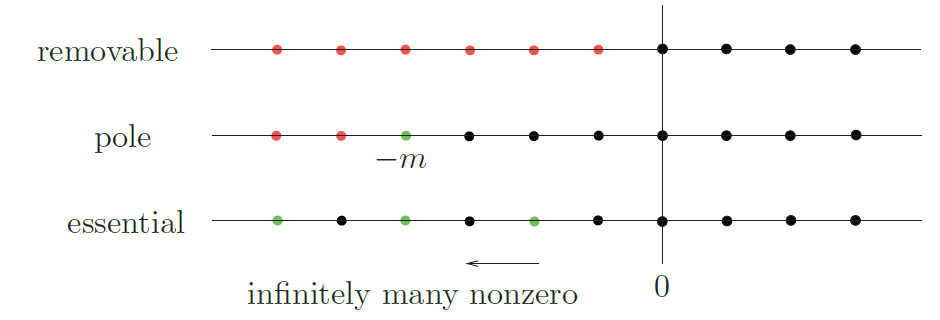
\includegraphics[width=0.8\textwidth]{./SaltChapter/fig-4-0-8}
\end{center}
%\caption{$\mathbb C$에 정의된 제곱급수의 수렴영역}
%\label{fig-4-0-3}
\end{figure*}

{\bf 증명}

(1) \fbox{$z_0$는 제거가능한 특이점이다. 
$\Rightarrow$ 모든 $n<0$에 대하여 $c_n=0$.}

$z_0$가 제거가능한 특이점이라고 가정하자.
그러면 $f$는 $|z-z_0|<R$에 정의된 복소해석함수 $F$로 확장할 수 있다.
$F$의 테일러 급수 전개는
\[
F(z) = \sum_{n=0}^\infty  \tilde c_n (z-z_0)^n,\quad
|z-z_0| <R.
\]
특히, $0<|z-z_0| <R$에서
\[
f(z) = \sum_{n=0}^\infty  \tilde c_n (z-z_0)^n 
= \sum_{n\in\mathbb Z} c_n(z-z_0)^n
\]
이고 고정된 원환에서 로랑 급수 전개의 유일성으로부터
$n\ge0$에서 $c_n = \tilde c_n$이고,
$n<0$에서 $c_n=0$이다.

\fbox{ 모든 $n<0$에 대하여 $c_n=0$.
$\Rightarrow$ $z_0$는 제거가능한 특이점이다.}

모든 $n<0$에서 $c_n=0$이라고 가정하자. 그러면,
$0<|z-z_0|<R$에서
\[
f(z) = \sum_{n\in\mathbb Z} \tilde c_n (z-z_0)^n
= \sum_{n=0}^\infty  c_n (z-z_0)^n
\]
이고 $|z-z_0|<R$에서 $F$를
\[
F(z) = \sum_{n=0}^\infty  \tilde c_n (z-z_0)^n
\]
로 정의하면, $F$는 
$\{ z\in\mathbb C\,:\, |z-z_0|<R\}$에서 복소해석함수이다.
(왜냐하면 제곱급수로 정의되었기 때문에)
또한, $0<|z-z_0|<R$에서 $F=f$이다.

(2) $z_0$가 $m$차의 극이면,
\[
f(z) = \dfrac{c_{-m}}{(z-z_0)^m} + \cdots + \dfrac{c_{-1}}{z-z_0}
+ c_0 + \sum_{n=0}^\infty c_n(z-z_0)^n
\]
이고 $c_{-m} \ne 0$임을 증명해보자.
$z_0$가 $m$차의 극이라고 가정하자.
정리 \ref{thm-4-8}을 이용하면,
\[
\lim_{z\to z_0} (z-z_0)\left( (z-z_0)^m f(z) \right)
= \lim_{z\to z_0} (z-z_0)^{m+1} f(z) =0,
\]
이고 $(z-z_0)^m f(z)$는 $z_0$에서 제거가능한 특이점을 갖는다.
\[
(z-z_0)^mf(z) = (z-z_0)^m \sum_{n\in\mathbb Z}c_n(z-z_0)^n
= \sum_{n\in\mathbb Z}c_n(z-z_0)^{n+m}
\]
의 급수 전개에서 $z-z_0$의 차수가 음수인 항의 계수들은 모두 $0$이 되어야 한다.
즉, $0 = c_{-(m+1)} = c_{-(m+2)} = \cdots$.
따라서 $0<|z-z_0|<R$에 대하여
\begin{equation}\label{eq-4-6}
(z-z_0)^mf(z) = c_{-m} + c_{-m+1}(z-z_0) + c_{-m+2}(z-z_0)^2 + \cdots
\end{equation}
이므로,
\[
f(z) = \dfrac{c_{-m}}{(z-z_0)^m} + \cdots + \dfrac{c_{-1}}{(z-z_0)}
+ c_0 + c_1(z-z_0) + c_2(z-z_0)^2 + \cdots.
\]
또한, 
$c_{-m} + c_{-m+1}(z-z_0) + c_{-m+2}(z-z_0)^2 + \cdots$는 
복소해석함수이고, $z\to z_0$일 때 극한값 $c_{-m}$을 갖는다.
\[
\lim_{z\to z_0} (z-z_0)^mf(z) 
= \lim_{z\to z_0}  \left( 
c_{-m} + c_{-m+1}(z-z_0) + c_{-m+2}(z-z_0)^2 + \cdots \right) = c_{-m}.
\]
한편, $z_0$는 $m$차 극이므로, 
\[
\neg \left( \lim_{z\to z_0} (z-z_0)^mf(z) =0 \right).
\]
따라서 식 \eqref{eq-4-6}으로부터 $c_{-m} \ne 0$이다.

이제 
\[
f(z) = \dfrac{c_{-m}}{(z-z_0)^m} + \cdots + \dfrac{c_{-1}}{(z-z_0)}
+ c_0 + c_1(z-z_0) + c_2(z-z_0)^2 + \cdots
\]
이고 $c_{-m} \ne 0$를 가정하고 $z_0$가 $m$차 극임을 보이자.
어떤 $m\in \mathbb N$이 존재하여,
$c_{-m} \ne 0$이고, $n<-m$에 대하여 $c_n=0$이라고 가정하자.
그러면, 
$(z-z_0)^mf(z) = c_{-m} + c_{-m+1}(z-z_0) + c_{-m+2}(z-z_0)^2 + \cdots$이고
우변은 복소해석함수를 정의한다. 이를 $h$라 하자.
$\{z \in \mathbb C\,:\, |z-z_0| <R\}$에서
\begin{align*}
& \lim_{z\to z_0} (z-z_0)^m f(z) = \lim_{z\to z_0} h(z) = h(z_0) = c_{-m} \ne0,\\
& \lim_{z\to z_0} (z-z_0)^{m+1}f(z) = 0 \cdot c_{-m} = 0.
\end{align*}
따라서, 정리 \ref{thm-4-8}에 의해 $z_0$는 $m$차 극이다.

(3) 본질적 특이점은 제거가능한 특이점 또는 극이 아닌 경우를 뜻하므로
앞의 두 경우의 증명으로부터 쉽게 도출된다.
\hfill $\square$

다시 예제 \ref{example-4-14}를 돌아보자.

\begin{saltexample}[label=example-4-16]{}{}

\begin{itemize}
\item[(1)] $z\ne0$에 대하여
\[
\dfrac{\sin z}z = \dfrac 1z\left( z - \dfrac{z^3}{3!} + \dfrac{z^5}{5!} - \cdots
\right) =1 - \dfrac{z^2}{3!} + \dfrac{z^4}{5!} - \dfrac{z^6}{7!} + \cdots.
\]
로랑 급수에서 $z$의 음의 지수 항이 나타나지 않기 때문에
$0$은 제거가능한 특이점이다.
\item[(2)] $z\ne0$에 대하여 
\[
\dfrac1{z^3} = \cdots + 0 + \dfrac1{z^3} + 0 + \cdots.
\]
$c_{-3}=1 \ne 0$이고 $0=c_{-4} = c_{-5} = \cdots$이다.
따라서 $\dfrac1{z^3}$은 $0$에서 $3$차의 극을 갖는다.
\item[(3)] $z\ne0$에 대하여 
\[
\exp \dfrac1z = 1 + \dfrac1{1!z} + \dfrac1{2!z^2} + \dfrac1{3!z^3} + \cdots
\]
무한이 많은 음의 인덱스 (실제로 모든) $n$에서 $0$이 아니므로
\[
c_{-n} = \dfrac1{n!} \ne 0
\]
$0$은 $\exp \dfrac1z$의 본질적 특이점이다.
\hfill $\diamondsuit$
\end{itemize}
\end{saltexample}

\begin{salt_exercise}\label{ex-4-30}
영역 $D$에 정의된 복소해석함수 $f$가 $D$에서 유일한 근으로
$m$중근 $z_0$를 갖는다고 하자.
함수 $z\mapsto 1/f(z)$는 $z_0$에서 $m$차 극을 가짐을 보여라.
\end{salt_exercise}

\begin{salt_exercise}\label{ex-4-31}
$D$가 $z_0$를 중심으로 하는 원판이고, 
$D\setminus \{z_0\}$에 정의된 함수 $f$는 함수값이 $0$이 되지 않으며
$z_0$에서 $m$차 극을 갖는다고 하자. 
함수 $z\mapsto 1/f(z)$는 $D$에 정의된 복소해석함수 $g$로 확장될 수 있으며
$g$는 $z_0$에서 $m$중근을 가짐을 보여라.
\end{salt_exercise}

\begin{salt_exercise}\label{ex-4-32}
영역 $D$와  $z_0\in D$에 대하여
$f$는 $z_0$에서 $m$차 극을 가지며 다음과 같은 로랑 급수 전개가 가능하다고 하자.
\[
f(z) = \sum_{n\in\mathbb Z} c_n(z-z_0)^n,\quad
0<|z-z_0|<R,
\]
단, $R$은 양의 상수이다. 다음 식이 성립함을 보여라.
\[
c_{-1} = \dfrac1{(m-1)!}\lim_{z\to z_0} \dfrac{d^{m-1}}{dz^{m-1}}
\left( (z-z_0)^m f(z) \right).
\]
\end{salt_exercise}

\begin{salt_exercise}\label{ex-4-33}
참 또는 거짓을 밝혀라.
\begin{itemize}
\item[(1)] $f$의 로랑 급수가 $z^{-1} + c_0 + c_1z + \cdots$가
원점을 중심으로 하는 어떤 뚫린원판에서 수렴한다면, $f$는 $0$에서 극을 갖는다.
\item[(2)] 하나의 함수가 수렴하는 원환의 선택에 따라 $z_0$를 중심으로 다른
로랑 급수를 가질 수 있다.
\item[(3)] $f$가 $z_0$에서 고립 특이점을 갖는다면, 
$z_0$를 중심으로 하는 로랑 급수는 원환 $0<|z-z_0|<R$에서 수렴한다.
\item[(4)] $f$의 로랑 급수가 원환 $R_1 <|z-z_0| <R_2$에서
실제로 테일러 급수가 되면 ($z-z_0$의 음의 지수 항이 없다면),
이 급수는 실제로 (적어도) 원판 $|z-z_0|<R_2$에서 수렴한다.
\item[(5)] 앞의 결과가 맞다면, $f$가 원판 $|z-z_0|<R_2$에서
특이점이 있더라도 제거가능한 특이점만 존재하며 
이 원판에서 복소해석함수로 간주할 수 있다.
\end{itemize}
\end{salt_exercise}

\begin{salt_exercise}\label{ex-4-34}
다음 함수들이 $0$에서 특이점을 갖는다면 어떤 종류인지 판정하라.
복소해석함수이거나 고립 특이점을 갖는 함수이면
뚫린원판 $0<|z|<R$에서 수렴하는 급수로 전개하라.
\[
\sin z, \quad \sin \dfrac1z,\quad \dfrac{\sin z}z,
\quad \dfrac{\sin z}{z^2}, \quad \dfrac1{\sin \frac1z},
\quad z\sin \dfrac1z
\]
\end{salt_exercise}

\begin{salt_exercise}\label{ex-4-35}
참 또는 거짓을 밝혀라.
\begin{itemize}
\item[(1)] $\Lim_{z\to 0} \left| \exp \dfrac1z \right| = +\infty$.
\item[(2)] $f$가 $z_0$에서 $m$차 극을 가지면, 
$z_0$를 중심으로 하는 원판에서
$f - \dfrac{p}{(z-z_0)^m}$가 복소해석함수가 되게 하는
다항식 $p$가 존재한다.
\item[(3)] $f$가 $0$의 근방에서 복소해석함수이면,
$n>m$일 때 $\dfrac f{z^n}$이 $0$에서 극을 갖는 정수 $m$이 존재한다.
\item[(4)] $z_0$에서 $f$, $g$가 각각 $m_f$차, $m_g$차 극을 갖는다면,
점별 곱으로 정의된 함수 $f\cdot g$는 $z_0$에서 $m_f+m_g$차 극을 갖는다.
\end{itemize}
\end{salt_exercise}

\begin{salt_exercise}\label{ex-4-36}
두 본질적 특이점 $0$과 $1$을 제외한  $\mathbb C$ 에서
복소해석함수인 예를 들면?
\end{salt_exercise}

\begin{salt_exercise}\label{ex-4-37}
함수 $f(z) = 1/(z-1)$은 $0$에서 특이점을 갖지 않음은 분명하다.
그런데 $|z|>1$에서 로랑 급수가 $z^{-1} + z^{-2} + z^{-3} + \cdots$이므로
무한이 많은 $z$의 음의 차수 항이 $0$이 아기 때문에
$0$은 $f$의 본질적 특이점으로 오해할 수 있다. 
이 주장에서 무엇이 잘못되었는지 찾아라.
\end{salt_exercise}

\begin{salt_exercise}\label{ex-4-38}
증명 또는 반증하라:
$z_0$에서 $f$와 $g$가 각각 극과 본질적 특이점을 찾는다면,
$fg$는 $z_0$에서 본질적 특이점을 갖는다.
\end{salt_exercise}

\subsection{본질적 특이점 근방에서의 역동적 변화}

이제 본질적 특이점 $z_0$의 근방에서 함수 $f$의
``역동적'' 변화를 보여주는 결과를 살펴보자. 
임의의 복소수 $w$와 $\epsilon>0$, 
$z_0$를 중심으로 하는 임의의 작은 뚫린원판 $\Delta$이
주어졌을 때, 
$f(z)$와 $w$의 거리가 $\epsilon$보다 작은 점 $z$가
$\Delta$에 존재한다. 따라서
본질적 특이점을 중심으로 하는 임의의 뚫린원판의 상(image)은
$\mathbb C$에서 조밀하다.
다른 표현으로는, 본질적 특이점 $z_0$의 임의의 근방에서
함수 $f$는 임의의 복소수에 가까이 다가갈 수 있다.

\begin{salttheorem} [카소라티-바이어스트라스] {}{}
\footnote{
이 결과는 바이어스트라스(Weierstrass)에 의해
1876년 (독일어로) 그리고
소콧스키(Sokhotski)에 의해 1873년(러시아어로) 발표되었다.
따라서 러시아 문헌에서는 소콧스키 정리로
서양에서는 바이어스트라스 정리로 불렸다. 
같은 정리는 이미 1868년 카소라티(Casorati)가 출판하였고,
1859년 Briot와 Bouquet의 책의 초판에도 소개되었다.
하지만, 이들은 1875년 개정판을 만들면서 정리를 삭제해버렸다.
} \label{thm-4-10}
$z_0$가 $f$의 본질적 특이점이하고 하자. 그러면,
\begin{itemize}
\item[(1)] 임의의 복소수 $w$,
\item[(2)] 임의의 $\delta>0$,
\item[(3)] 임의의 $\epsilon>0$에 대하여,
\end{itemize}
$z\in\mathbb C$가 존재하여
$|z-z_0| <\delta$와 $|f(z) - w| < \epsilon$을 만족한다.
\end{salttheorem}

\begin{figure*}[h!]
\begin{center}
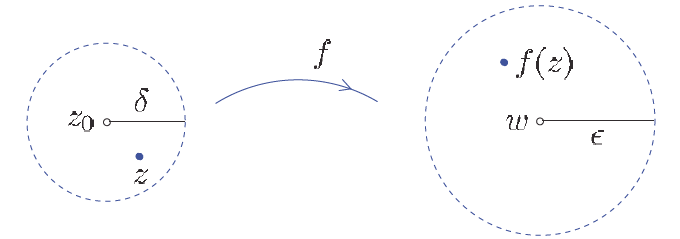
\includegraphics[width=0.6\textwidth]{./SaltChapter/fig-4-0-9}
\end{center}
%\caption{$\mathbb C$에 정의된 제곱급수의 수렴영역}
%\label{fig-4-0-3}
\end{figure*}

{\bf 증명}

증명의 결과를 부정하자.
그러면 $w\in\mathbb C$, $\epsilon>0$, $\delta>0$이 존재하여
$z\in D:= \{ z\in\mathbb C\,:\, 0<|z-z_0|<\delta\}$일 때
$|f(z) -w| \ge \epsilon$를 얻는다.
이제  $z\in D$에 대하여
\[
g(z) = \dfrac1{f(z)-w}
\]
로 정의하면, $g$는 복소해석함수이고,
\[
0\le |g(z)| = \dfrac1{|f(z)-w|} \le \dfrac1\epsilon, \quad
z\in D
\]
이므로 
$\Lim_{z\to z_0} (z-z_0)g(z) = 0$이다.
따라서 $g$는 제거가능한 특이점 $z_0$를 갖는다.
이 함수를 확장한 것도 $g$로 쓰기로 하자.
$g$가 $z_0$에서 $m$중근을 갖는다고 하면
($g(z_0)\ne0$이면 $m=0$으로 설정한다)
$g(z) = (z-z_0)^m h(z)$로 쓸 수 있다.
여기서, $h$는 $D$에 정의된 복소해석함수로 $h(z_0)\ne0$이다.
그러면, $0 < |z-z_0| < \delta$에 대하여
\begin{align*}
(z-z_0)^{m+1} f(z)
&= (z-z_0)^{m+1}(f(z) -w + w) \\
&= (z-z_0)^{m+1} \dfrac1{g(z)} + (z-z_0)^{m+1}\cdot w \\
&= \dfrac{z-z_0}{h(z)} + (z-z_0)^{m+1}\cdot w \\
& \stackrel{z\to z_0}{\longrightarrow}
\dfrac0{h(z_0)} + 0 \cdot w = 0.
\end{align*}
따라서, $f$는 $z_0$에서 제거가능한 특이점을 갖거나($m=0$일 때),
극($m\in\mathbb N$일 때)을 갖는다.
따라서 $z_0$는 $f$의 본질적 특이점이 되지 못하므로
모순이 되어 증명이 끝난다. \hfill $\square$

\begin{saltexample}[label=example-4-17]{}{}
함수 $\exp (1/z)$는 $0$에서 본질적 특이점을 갖는다.
$0$의 임의의 근방에서
$0$이 아닌 모든  $w$ ($=\rho \exp(i\theta)$, $\rho, \theta \in \mathbb R$)
를 함수값으로 가짐을 보일 것이다.
이를 위해 $z= r\exp(it)$라 하면,
\[
\exp \dfrac 1z = \exp \left( \dfrac {\cos t}r  - i \dfrac{\sin t}r\right) 
= \rho e^{i\theta}
\]
를 풀어야 한다.
절대값을 취하는 방법으로 
\[
\dfrac{\cos t}r = \log \rho,
\]
한편 편각을 비교하면
하나의 해는 
\[
- \dfrac{\sin t}r = \theta.
\]
를 풀어서 얻을 수 있다.
$(\cos t)^2 + (\sin t)^2 =1$을 이용하면,
\[
r = \dfrac1{\sqrt{(\log \rho)^2 + \theta^2}}
\]
과 
\[
\tan t = - \dfrac{\theta}{\log \rho}
\]
를 얻는다. $\theta$가 $2\pi$ 주기를 가지므로
$2\pi$의 정수배를 더해도 $w$는 변하지 않는다. 
이로부터 $r$을 원하는 만큼 작게 만들 수 있다.
\hfill $\diamondsuit$
\end{saltexample}

이 예제는 카소라티-바이어스트라스 정리가 얼마나 강력한 것인지 보여준다.
피카드는 본질적 특이점을 중심으로 하는 임의의 뚫린원판의 상은
복소평면에서 기껏해야 한 점을 제외한 집합이 됨을 보였다.
우리는 예제에서 함수의 상이 $w=0$를 제외한 집합이 됨을 확인하였다.
피카드 정리는 이 책의 범위를 벗어나며, [Conway (1978)]을 참고하라.

\begin{salt_exercise}\label{ex-4-39}
카소라티-바이어스트라스 정리를 이용하여
$f$가 $z_0$에서 본질적 특이점을 가지고,
$w$가 임의의 복소수라고 하면,
\[
\Lim_{n\to \infty} z_n = z_0,
\quad
\Lim_{n\to\infty} f(z_n) = w.
\]
를 만족하는 복소수열 $z_1, z_2, z_4, \ldots$이 존재함을 보여라.
\end{salt_exercise}

\section{유수 정리}

$D$가 영역일 때
복소해석함수 $f:D\setminus \{z_0\}\to \mathbb C$가
$z_0$에서 고립 특이점을 갖는다고 하자.
\[
f(z) = \sum_{n\in\mathbb Z} c_n (z-z_0)^n,\quad
0<|z-z_0|<R.
\]
이 때, $c_{-1}$을 $z_0$에서 $f$의 {\bf 유수}(residue)라고 하며,
\[
\res(f,z_0)
\]
로 쓴다.
왜 이런 이름을 붙였을까?
일상적인 언어에서 유수(residue)는 남은 것(left over)을 뜻한다.
위의 $c_{-1}$도 다음과 같이 남은 것으로 생각할 수 있다.
\[
2\pi i c_{-1} = \int_{C_r} \dfrac{f(z)}{(z-z_0)^{-1+1}}dz
= \int_{C_r} f(z)dz 
= \int_{C_r} \left( \sum_{n\in\mathbb Z}c_n(z-z_0)^n\right) dz,
\]
여기서 $C_r$은 $C_r(t) = z_0 + r\exp(it)$ ($t\in[0,2\pi]$)이고
$r<R$이다.
\[
\int_{C_r} \left( c_n(z-z_0)^n \right) dz = 
\begin{cases}
0, & n\ne -1, \\
2\pi i c_{-1}, & n= -1
\end{cases}
\]
로부터 $f$의 로랑 급수 전개를 (수렴성은 따지지 않고) 항별 적분이 가능하다고 
상상해보면 적분 결과로 $2\pi i c_{-1}$만 남는다.

유수가 무엇이길래 큰 소란일까? 등식
\[
2\pi i c_{-1}= \int_{C_r} f(z)dz 
\]
은 경로적분의 계산을 $z_0$에서 $f$의 유수를 계산하는 방법으로 구할 수 있음을 뜻한다.
(물론 $f$의 로랑 급수로부터 계수 $c_{-1}$을 구하는 것이 필요하다.)
따라서 $c_{-1}$을 쉽게 구하는 방법이 있다면
경로 $C_r$과 $D\setminus\{z_0\}$-호모토픽한 임의의 닫힌경로 $\gamma$를 따르는 적분을
다음과 같이 계산할 수 있다.
\begin{equation} \label{eq-4-7}
\int_\gamma f(z)dz \left( = \int_{C_r} f(z)dz \right) = 2\pi i c_{-1}.
\end{equation}
연습문제 \ref{ex-4-32}의 결과에서 
$z_0$가 $m$-중극 일 때,
$c_{-1}$을 계산하는 공식을 얻는다.
\[
c_{-1} = \dfrac1{(m-1)!}\lim_{z\to z_0} \dfrac{d^{m-1}}{dz^{m-1}}
\left( (z-z_0)^m f(z) \right).
\]
계산하기 불편한 실적분의 경우 때로는
적절한 복소해석함수 $f$의 $\gamma$를 따른 경로적분으로 변형한 다음
유수를 이용하여 경로적분을 구한다.
그러면 원하는 실적분의 값을 얻을 수 있다.
관련하여 다음 예제를 보자.

\begin{saltexample}[label=example-4-18]{}{}
실적분
\[
\int_0^{2\pi} \dfrac1{5 + 3\cos\theta} d\theta
\]
를 계산해보자.
우선 이 적분을 원을 따르는 경로적분으로 변형한다.
$z:=\exp(i\theta)$라 하면
\[
\cos\theta = \dfrac{\exp(i\theta) + \exp(-i\theta)}2 
= \dfrac{z+ \dfrac1z}2 = \dfrac{z^2+1}{2z}.
\]
$\gamma$를 중심이 $0$이고 반지름 $1$인 원형경로로 잡으면,
\[
\gamma(\theta) = \exp(i\theta), \quad \theta \in [0,2\pi],
\]
이고 $\gamma'(\theta) d\theta = i\exp(i\theta)d\theta = izd\theta$이다.
따라서
\[
\int_0^{2\pi} \dfrac1{5 + 3\cos\theta} d\theta
= \int_\gamma \dfrac1{5+3\cdot\left(\dfrac{z^2+1}{2z}\right)}
\dfrac1{iz}dz
= \int_\gamma - \dfrac{2i}{(3z+1)(z+3)}dz.
\]
\[
f(z) = - \dfrac{2i}{(3z+1)(z+3)}
\]
로 정의하면 $f$는 $-1/3$과 $-3$에서 극을 가지며,
두 극의 차수는 모두 $1$이고,
그 중에서 $-1/3$만 닫힌경로 $\gamma$의 내부에 존재한다.
따라서
\[
\int_0^{2\pi} \dfrac1{5 + 3\cos\theta} d\theta
= \int_\gamma f(z)dz = 2\pi i \cdot \res\left(f, -\dfrac13\right).
\]
$c^{-1}$의 값은? 중심 $-1/3$의 뚫린원판에서
\[
f(z) = \dfrac{c_{-1}}{z+ \dfrac13} + c_0 + c_1\left(z + \dfrac13\right)
+ c_2\left(z+\dfrac13\right)^2 + \cdots
\]
이고 $\left(z+\dfrac13\right) f(z) = c_{-1} + c_0\left(z + \dfrac13\right) + \cdots$이다.
따라서
\[
c_{-1} = \lim_{z\to -1/3} \left(z+\dfrac13\right) f(z)
= \lim_{z\to -1/3} - \dfrac{2i}{3(z+3)} = - \dfrac i4.
\]
결론적으로 $\dint_0^{2\pi} \dfrac1{5 + 3\cos\theta} d\theta = \dfrac\pi2$이다.
\end{saltexample}

좀 더 일반화하면, $f$가 $D$에서 유한개의 극을 갖는 경우,
적분을 식 \eqref{eq-4-7}과 유사한 방법으로 계산할 수 있다.
이를 다음 정리에서 다룬다.

\begin{salttheorem} [유수정리] {}{} \label{thm-4-11}

\begin{itemize}
\item[(1)] $D$가 영역이고,
\item[(2)] $f$가 $D\setminus \{p_1, \ldots, p_K\}$에서 해석적이고,
\item[(3)] $f$가 $p_1, \ldots, p_K$에서 각각 $m_1, \ldots, m_K$-중극을 가지며,
\item[(4)] $\gamma$는 $D\setminus \{p_1, \ldots, p_K\}$의 닫힌경로이고,
\item[(5)] $\gamma$는 각각의 $k=1,\ldots, K$에 대하여
$C_k$와 $D\setminus\{p_k\}$-호모토픽하다.
여기서, $C_k$는 중심이 $p_k$이고 $C_k$의 내부는 $D$에 속하며 
내부의 극은 $p_k$뿐이다.
\end{itemize}
그러면, $\dint_\gamma f(z)dz = 2\pi i \Sum_{k=1}^K \res(f,p_k)$이다.
\end{salttheorem}

\begin{figure*}[h!]
\begin{center}
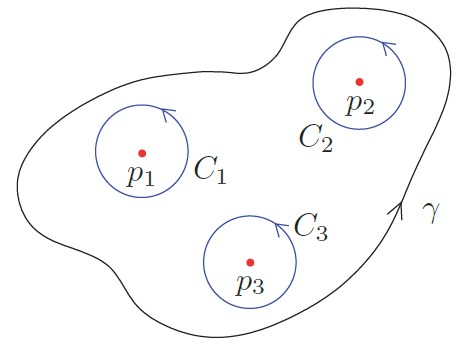
\includegraphics[width=0.35\textwidth]{./SaltChapter/fig-4-0-10}
\end{center}
%\caption{$\mathbb C$에 정의된 제곱급수의 수렴영역}
%\label{fig-4-0-3}
\end{figure*}

{\bf 증명.}

각각의 $k=1,\ldots, K$에 대하여,
적당한 $R_k>0$가 존재하여 $0<|z-p_k|<R_k$에서
\[
f(z) = \sum_{n=1}^{m_k} c_{-n,k} (z-p_k)^{-n}
+ \sum_{n=0}^\infty c_{n,k} (z-p_k)^n = f_k(z) + h_k(z)
\]
로 쓸 수 있다. $z-p_k$의 음의 차수를 갖는 항은 $f_k$로, 
음이 아닌 차수 부분은 $h_k$로 표시하자.
$h_k$는 $|z-p_k|<R_k$에서 복소해석함수이고
$f_k$는 $\mathbb C\setminus\{p_k\}$에 정의되고
유일한 특이점으로 극 $p_k$를 갖는 유리함수이다.
따라서 $f-f_k$는 $p_k$를 포함한 작은 원판에서 복소해석함수이다.
$g:= f - (f_1+\cdots + f_K)$라고 하자.
$k\in \{1,\ldots, K\}$를 고정하면
\[
g = (f-f_k) = \sum_{j\ne k} f_j
\]
로 쓸 수 있다.
$f-f_k$와 $j\ne k$인 $f_j$는 모두 $p_k$를 중심으로 하는 작은 원판에서
복소해석함수이다. 그러므로 $g$는 $D$에서 복소해석함수이다.
$\gamma$는  $p_1$을 중심으로 하는 원 $C_1$과 $D\setminus\{p_1\}$-호모토픽하므로
코시 적분정리에서
\[
\int_\gamma g(z)dz  = 0
\]
이고, $\dint_\gamma \left( f - (f_1+\cdots + f_K) \right) dz = 0$이다.
코시 적분정리를 다시 적용하면,
\[
\int_\gamma f_k(z)dz = \int_{C_k} f(z)dz = 2\pi i c_{-1,k},
\quad k=1,\ldots, K
\]
이므로
\[
\int_\gamma f(z)dz  = \sum_{k=1}^K \int_\gamma f_k(z)dz
= \sum_{k=1}^K 2\pi i c_{-1,k} = 2\pi i \sum_{k=1}^K \res(f,p_k).
\]

\begin{salt_exercise}\label{ex-4-40}
아래 그림과 같은 경로 $\gamma$를 따라
적분 $\dint_\gamma \dfrac{\Log(z)}{1+\exp z} dz$를 계산하라.
\begin{figure*}[h!]
\begin{center}
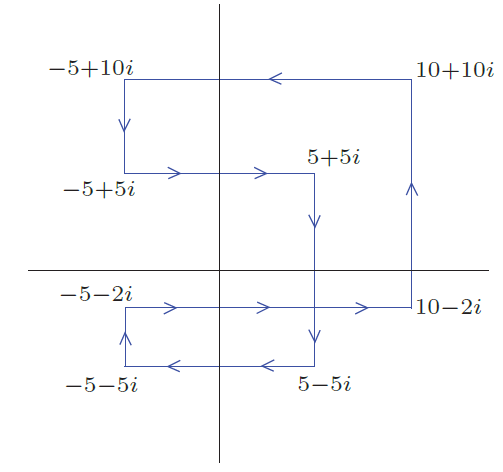
\includegraphics[width=0.33\textwidth]{./SaltChapter/fig-4-0-11}
\end{center}
%\caption{$\mathbb C$에 정의된 제곱급수의 수렴영역}
%\label{fig-4-0-3}
\end{figure*}
\end{salt_exercise}

{\bf 유수정리를 이용한 유리함수의 실적분}

앞에서 언급한 바와 같이
유수정리는 경로적분에 사용될 수 있지만
때로는 실적분을 쉽게 계산하기 위해 사용될 수도 있다.
다음 유형의 실적분을 생각하자.
\[
\int_{-\infty}^\infty f(x)dx.
\]
이러한 적분은
적분구간이 유한하지 않기 때문에 특이적분(improper integral)이라 부르며
다음식에서 우변의 두 극한이 모두 존재할 때 정의된다.
\begin{equation}\label{eq-4-8}
\int_{-\infty}^\infty f(x)dx = \lim_{a\to-\infty} \int_a^0 f(x) dx
+ \lim_{b\to+\infty} \int_0^b f(x)dx.
\end{equation}
두 극한이 모두 존재하는 경우 적분값은 아래와 같이 쓸 수도 있다.
\begin{equation} \label{eq-4-9}
\int_{-\infty}^\infty f(x)dx = \lim_{r\to+\infty} \int_{-r}^r f(x) dx.
\end{equation}
식 \eqref{eq-4-9}의 우변의 극한이 존재하면 
이를 적분의 {\bf 코시 주치}(Cauchy principal value)라고 한다.
코시 주치는 존재하지만 특이적분은 존재하지 않을 수 있다.
예를 들면, $\dint_0^b xdx = \dfrac{b^2}2$이므로
\[
\lim_{r\to+\infty} \int_{-r}^r x dx = 
\lim_{r\to+\infty} \left( \dfrac{r^2}2 - \dfrac{r^2}2 \right) = 0
\]
이지만, 특이적분은 존재하지 않는다.

식 \eqref{eq-4-8}에서 피적분함수가 유리함수이고
분모가 모든 실수 $x$에 대하여 $0$이 되지 않으며
분모의 차수는 분자의 차수보다 적어도 $2$ 이상 큰 경우를 생각하자.
그러면 식 \eqref{eq-4-8}의 극한이 존재한다. 따라서
적분값의 계산은 식 \eqref{eq-4-9}로 시작하면 된다.

그림 \ref{fig-4-4}의 경로 $\gamma$를 따르는 적분
$\dint_\gamma f(z)dz$를 생각하자.

\begin{figure}[h!]
\begin{center}
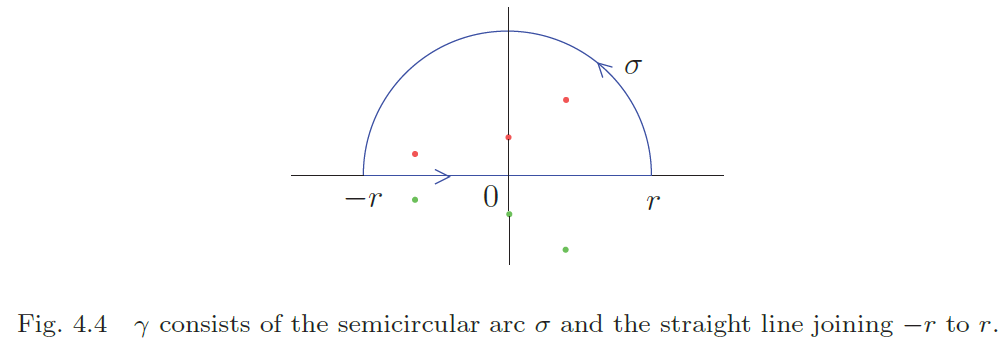
\includegraphics[width=0.7\textwidth]{./SaltChapter/fig-4-4}
\end{center}
\caption{반원 $\sigma$와 $-r$과 $r$을 잇는 직선으로 구성된 경로 $\gamma$}
\label{fig-4-4}
\end{figure}

$f$가 유리함수이므로 $z\mapsto f(z)$는 상반평면에서 (기껏해야) 유한개의 극을 가지므로,
$r$을  충분히 크게 잡으면 상반평면의 모든 극을 $\gamma$의 내부에 포함할 수 있다.
유수정리에 의하여
\[
\int_\gamma f(z)dz = \int_\sigma f(z)dz + \int_{-r}^r f(x)dx
= 2\pi i \Sum_{k: \Im(p_k)>0} \res(f,p_k),
\]
여기서, 상반평면에 있는 극에 대해서만 합을 계산한다.
이로부터
\[
\int_{-r}^r f(x)dx = 2\pi i \Sum_{k: \Im(p_k)>0} \res(f,p_k)
- \int_\sigma f(z)dz.
\]
$r$이 커짐에 따라 반원 $\sigma$를 따라 적분한 값이 $0$에 가까워짐을 보일 수 있다.
$f$의 분모와 분자의 차수가 $2$ 이상이므로, 
\[
|f(z)| \le \dfrac M{|z|^2} \quad (|z|>r_0)
\]
를 만족하는 $M$, $r_0$가 존재한다.
따라서 $r>r_0$에 대하여
\[
\left| \int_\sigma f(z)dz \right| \le \dfrac  M{r^2} \pi r = \dfrac {M\pi}r.
\]
결론적으로
$\Lim_{r\to+\infty} \dint_\sigma f(z)dz = 0$이 되어
\[
\int_{-\infty}^\infty f(x)dx
= 2\pi i \Sum_{k: \Im(p_k)>0} \res(f,p_k).
\]

이 방법을 예제에 적용해보자.

\begin{saltexample}[label=example-4-19]{}{}
$\dint_0^ \infty \dfrac1{1+x^4}dx = \dfrac{\pi}{2\sqrt{2}}$를 계산해보자.
함수 $f$를  $f(z) = \dfrac1{1+z^4}$라 정의하면 $4$개의 극을 갖는다.
\[
p_1 = \exp\left(\dfrac{\pi i}4\right), \quad
p_2 = \exp\left(\dfrac{3\pi i}4\right), \quad
p_3 = \exp\left(\dfrac{5\pi i}4\right), \quad
p_4 = \exp\left(\dfrac{7\pi i}4\right).
\]
%\begin{figure*}[h!]
\begin{center}
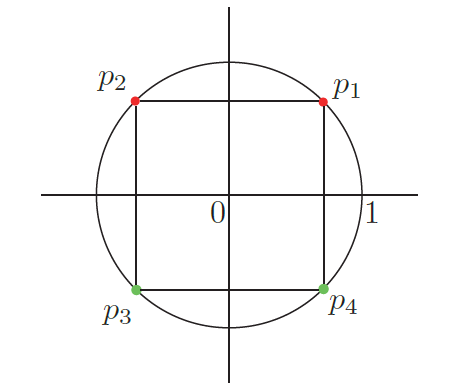
\includegraphics[width=0.3\textwidth]{./SaltChapter/fig-4-0-12}
\end{center}
%\caption{$\mathbb C$에 정의된 제곱급수의 수렴영역}
%\label{fig-4-0-3}
%\end{figure*}
\end{saltexample}
처음 두 개의 극은 상반평면에 있다. 유수를 계산하면,
\begin{align*}
\res(f,p_1) &= \lim_{z\to p_1} \dfrac{z-p_1}{1+z^4} 
= \lim_{z\to p_1} \dfrac1{\dfrac{(1+z^4) - (z+p_1^4)}{z-p_1}} \\
&= \dfrac1{\dfrac{d}{dz}(1+z^4)\Big|_{z=p_1}} = \dfrac1{4p_1^3}
= - \dfrac14 \exp\left(\dfrac{\pi i}4\right),
\end{align*}
\begin{align*}
\res(f,p_2) &= \lim_{z\to p_2} \dfrac{z-p_2}{1+z^4} 
= \lim_{z\to p_2} \dfrac1{\dfrac{(1+z^4) - (z+p_2^4)}{z-p_2}} \\
&= \dfrac1{\dfrac{d}{dz}(1+z^4)\Big|_{z=p_2}} = \dfrac1{4p_2^3}
= \dfrac14 \exp\left(-\dfrac{\pi i}4\right).
\end{align*}
따라서
\[
\dint_{-\infty}^ \infty \dfrac1{1+x^4}dx
= 2\pi i \left( - \dfrac14 \exp\left(\dfrac{\pi i}4\right)
+ \dfrac14 \exp\left(-\dfrac{\pi i}4\right) \right)
= \pi \sin \dfrac\pi 4 = \dfrac\pi{\sqrt{2}}.
\]
$f$가 우함수 (모든 $x\in\mathbb R$에 대하여 $f(x)=f(-x)$)이므로
\[
\dint_{-\infty}^ \infty \dfrac1{1+x^4}dx = \dfrac12 
\dint_0^ \infty \dfrac1{1+x^4}dx = \dfrac{\pi}{2\sqrt{2}}.
\]
\hfill $\diamondsuit$

피적분함수가 유리함수가 아닌 색다른  유형의 계산 예를 살펴보자.

\begin{saltexample}[label=example-4-20]{[프레넬 적분]}{} \footnote{
이 적분은 광학에서 회절현상을 설명하기 위해 사용된다.
}
\[
\int_0^\infty \cos(x^2) dx =  \int_0^\infty \sin(x^2) dx 
= \dfrac{\sqrt{\pi}}{2\sqrt{2}}
\]
를 계산해보자.
경로 $\gamma$가 아래 그림과 같을 때
경로적분 $\int_\gamma \exp(iz^2) dz$을 생각하자.

%\begin{figure*}[h!]
\begin{center}
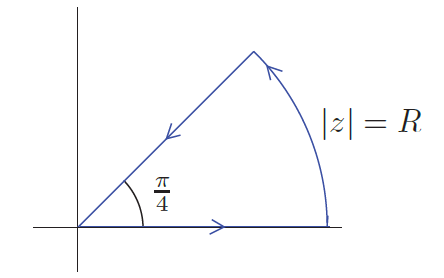
\includegraphics[width=0.3\textwidth]{./SaltChapter/fig-4-0-13}
\end{center}
%\caption{$\mathbb C$에 정의된 제곱급수의 수렴영역}
%\label{fig-4-0-3}
%\end{figure*}

$\exp(iz^2)$은 전해석함수이므로
코시 적분정리에 의해
\begin{align*}
0 &= \int_\gamma \exp(iz^2) dz \\
& = \int_0^R \exp(ix^2)dx 
+ \int_0^{\frac\pi4} \exp(iR^2\exp(2i\theta))iR\exp(i\theta)d\theta \\
&\quad\quad 
- \int_0^R \exp\left( it^2\exp\left(i\dfrac\pi2\right)\right) 
\exp\left( i\dfrac\pi4\right)dt.
\end{align*}
$R\to\infty$일 때, 가운데 적분값은 $0$으로 수렴함을 보이자.
우선 
\begin{align*}
\left|  \exp(iR^2\exp(2i\theta))iR\exp(i\theta)  \right|
&= \left| R\exp\left(R^2(i\cos(2\theta)) - \sin(2\theta))\right) \right| \\
&= Re^{-R^2\sin(2\theta)}.
\end{align*}
그림 \ref{fig-4-5}를 보면 $0<t<\dfrac\pi2$인 $t$에 대하여
\[
\dfrac2\pi \le \dfrac{\sin t}t
\]
가 성립한다. 왜냐하면, 호 $PAQ$의 길이는 $2t$이고,
반원 $PBQ$의 길이 $\pi\sin t$보다 짧기 때문이다.
(다른 방법으로 $t\mapsto \sin t$는 $[0,\pi]$에서 
두번 미분하면 $-\sin t$로 음수가 되므로 위로 볼록하다.
따라서 $\sin t$의 그래프는 두점 $(0,0)$과 $(\pi/2,1)$을 잇는 직선 $2t/\pi$보다 위에 있다.)


%\begin{figure*}[h!]
\begin{center}
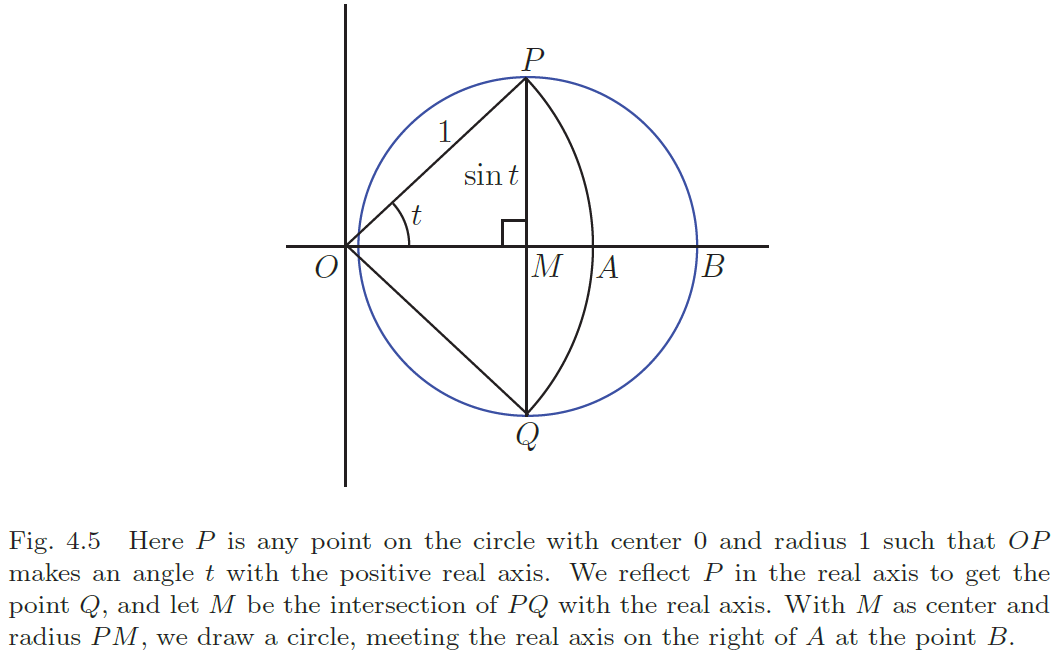
\includegraphics[width=0.7\textwidth]{./SaltChapter/fig-4-5}
\end{center}
\captionof{figure}{원점을 중심으로 반지름 $1$인 원 위의 한점 $P$를 잡고 $OP$가
실수축의 양의 방향과 이루는 각도를 $t$라 하자. $P$를 실수축에 대칭시켜 $Q$를
잡고, $M$을 $PQ$와 실수축의 교점이라 하자. $M$을 중심으로 반지름 $PQ$인 원을 그릴 때
$A$의 오른쪽에서 실수축과 만나는 점을 $B$라고 정한다. }
\label{fig-4-5}
%\end{figure*}
이 부등식에 $t=2\theta$를 대입하면,
\[
\left| \exp(iR^2\exp(2i\theta))iR\exp(i\theta) \right|
= Re^{-R^2\sin(2\theta)} \le Re^{-R^2\frac{4\theta}\pi}
\]
이므로
\[
\left| \int_0^{\frac\pi4} \exp(iR^2\exp(2i\theta))iR\exp(i\theta) d\theta\right|
\le R \int_0^{\frac\pi4} e^{-R^2\frac{4\theta}\pi}d\theta
= \dfrac\pi{4R}(1-e^{-R^2})
\]
은 $R\to +\infty$일 때 $0$으로 수렴한다.
따라서, 
\begin{align*}
\lim_{R\to+\infty} \int_0^R \exp(ix^2)dx 
&=  \lim_{R\to+\infty}\int_0^R  \exp\left( it^2\exp\left( i\dfrac\pi2 \right)\right)
\exp\left(i\dfrac\pi4\right) dt \\
&= \dfrac{1+i}{\sqrt{2}} \int_0^\infty e^{-t^2}dt 
= \dfrac{(1+i)\sqrt{\pi}}{2\sqrt{2}}.
\end{align*}
마지막 계산을 위해 잘 알려진 공식\footnote{
\begin{align*}
I:=\dint_0^\infty e^{-x^2} dx\text{  라 하면, \ } 
I^2 &= \left(\dint_0^\infty e^{-x^2} dx\right)\left(\dint_0^\infty e^{-y^2} dy\right) 
= \int_0^\infty \int_0^\infty e^{-(x^2+y^2)}dxdy \\
&= \dint_0^{\frac\pi2} \int_0^\infty e^{-r^2}rdrd\theta = \dfrac\pi4.
\end{align*}
}을 사용했다.
\[
\dint_0^\infty e^{-x^2} dx = \dfrac{\sqrt{\pi}}2.
\]
실수부와 허수부를 나누어 비교하면, 원하는 결과를 얻는다.
\[
\int_0^\infty \cos(x^2) dx =  \int_0^\infty \sin(x^2) dx 
= \dfrac{\sqrt{\pi}}{2\sqrt{2}}.
\]
\end{saltexample}

\begin{salt_exercise}\label{ex-4-41}
적분 $\dint_0^{2\pi} \dfrac{\cos \theta}{5 + 4\cos\theta}d\theta$을 계산하라.
\end{salt_exercise}

\begin{salt_exercise}\label{ex-4-42}
다음 적분값을 구하라.
\begin{itemize}
\item[(1)] $\int_0^\infty \dfrac1{1+x^2} dx$.
\item[(2)] $\int_0^\infty \dfrac1{(a^2+x^2)(b^2+x^2)}dx$ (단, $a>b>0$).
\item[(3)] $\int_0^\infty \dfrac1{(1+x^2)^2}dx$.
\item[(4)] $\int_0^\infty \dfrac{1+x^2}{1+x^4}dx$.
\end{itemize}
\end{salt_exercise}

\begin{salt_exercise}\label{ex-4-43}
$n\in\mathbb N$, $C$는 $C(t)=\exp(i\theta)$, $\theta \in [0,2\pi]$일 때,
적분 $\dint_C \dfrac{\exp z}{z^{n+1}}dz$를 계산하고,
$\dint_0^{2\pi} e^{\cos\theta}\cos(n\theta - \sin \theta)d\theta = \dfrac{2\pi}{n!}$임을
유도하라.
\end{salt_exercise}

\begin{salt_exercise}\label{ex-4-44}
$f$가 $z_0$에서 차수 $1$의 근을 가지면, $1/f$는 $z_0$에서 차수 $1$의 극을 가진다.
$\res\left(\dfrac1f, z_0\right) = \dfrac1{f'(z_0)}$임을 증명하라.
\end{salt_exercise}

\begin{salt_exercise}\label{ex-4-45}
$\res\left(\dfrac1{\sin z}, k\pi\right) = (-1)^k$임을 증명하라.
\end{salt_exercise}

\begin{salt_exercise}\label{ex-4-46}
$n\ge0$일 때, 피보나치 수열의 $n$번째 항 $f_n$은 
점화식 $f_0=1, f_1=1, f_n = f_{n-1} + f_{n-2}$ ($n\ge2$)로 주어진다.
$F(z):= \Sum_{n=0}^\infty f_nz^n$이라 하자.
\begin{itemize}
\item[(1)] 점화식으로부터 모든 $n\in\mathbb N$에 대하여 $f_n\le 2^n$임을 보여라.
\item[(2)] $f_n\le 2^n$로부터 $F$의 수렴반경이 적어도 $1/2$ 이상임을 유도하라.
\item[(3)] $f_n$의 점화식을 이용하여 $F(z) = \dfrac1{1-z-z^2}$임을 보여라. \\
힌트: $zF(z)$와 $z^2F(z)$의 테일러 급수를 쓰고 더하라.
\item[(4)] $\res \left( \dfrac1{z^{n+1}(1-z-z^2)}, 0\right)=f_n$이 됨을 확인하라.
\item[(5)] 유수정리를 이용하여 다음을 증명하라.
\[
f_n = \dfrac1{\sqrt{5}} \left( \left(\dfrac{1+\sqrt{5}}2\right)^{n+1}
- \left(\dfrac{1-\sqrt{5}}2\right)^{n+1} \right).
\]
힌트: $\dfrac1{z^{n+1}(1-z-z^2)}$을 원점을 중심으로 반지름  $R$인 원의 둘레로
적분하고 $R\to+\infty$일 때 적분이 $0$으로 수렴함을 보여라.
\end{itemize}
\end{salt_exercise}

\section{참고}

\ref{sec-4-8}은 [Beck, Marchesi, Pixton, Sabalka (2008)]을 거의 따랐다.
연습문제 \ref{ex-4-11}, \ref{ex-4-24}, \ref{ex-4-33}, \ref{ex-4-35}, \ref{ex-4-36},
\ref{ex-4-37}, \ref{ex-4-38}, \ref{ex-4-39}는 [Franigan (1972)]에서 가져왔다.
연습문제 \ref{ex-4-14}는 [Volkovyski\u{\i}, Lunts, Aramanovich (1991)]을 인용하였다.
연습문제 \ref{ex-4-15},\ref{ex-4-25}는 [Rudin (1987)]에서
연습문제 \ref{ex-4-28}은 [Beck, Marchesi, Pixton, Sabalka (2008)]에서
연습문제 \ref{ex-4-40}은 [Ash and Novinger (2007)]에서 각각 인용하였다.











